\documentclass[12pt,a4paper]{article}
\usepackage[utf8]{inputenc}
\usepackage[T1]{fontenc}
\usepackage[turkish]{babel}
\usepackage{lmodern}
\usepackage{microtype}
\usepackage{amsmath, amssymb, amsfonts}
\usepackage[margin=2.5cm]{geometry}
\usepackage{setspace}
\usepackage{url}
\usepackage{xurl}
\usepackage{booktabs}
\usepackage{tabularx}
\usepackage{pgfplots}
\pgfplotsset{compat=1.18}
\usetikzlibrary{babel}

\onehalfspacing

\title{\textbf{Duran Sicimler Teoremi V: Eylül 2026 Navier--Stokes Girdap Tekilliğinin Elastik Sicim Gerilimiyle Durdurulması, $X \to 0$ Eksen Düzenlemesi ve Öz-Tutarlı Doyum Kanıtı} \\[0.3cm]
\large (Milenyum Girdap Çözümünün $(X,\eta,q)$ Benzerlik Koordinatlarında Analitik Türetimi, Kartezyen Eksen Regularizasyonu ve Yüksek Hassasiyetli Radau/DOP853 Sayısal Simülasyon Bulguları)}
\author{Fahri Meral}
\date{15 Ekim 2026}

\begin{document}
\shorthandoff{=}

\maketitle

\begin{abstract}
Eylül 2026'da yayımlanan \textit{Finite Time Blowup for Navier--Stokes} çalışması [1], üç boyutlu sıkıştırılamaz Navier--Stokes denklemlerinde durgunluktan başlayan düzgün bir akışkanın sonlu zamanda ($t \uparrow 1$, $\tau = 1-t \to 0$) eksenel simetrik bir girdap çekirdeği oluşturarak sonsuz hıza ($\|u_\theta^{(0)}\|_{L^\infty} \asymp \tau^{-1/2-h} \to \infty$) ulaştığını kanıtlamıştır. Söz konusu tekillik, benzerlik koordinatlarında $(X, \eta, q)$ merkezcil ivmenin yarattığı $\Pi_X^{(0)} = F(X,\eta)^2$ radyal basınç düşüşü ve $\Sigma_{r\theta} = -q^{-1-h} F(X,\eta) a(X,\eta)$ silindirik makaslama gerilmesi tarafından sürülmektedir [1, s. 8, 26, 27].

Bu çalışmada, \textit{Duran Sicimler Teoremi}'nin [2--5] öngördüğü ``boyutsal makaslama ve tekilliksiz çekirdek'' mekanizması doğrudan Eylül 2026 Navier--Stokes iç-çekirdek denklemlerine uygulanmakta, $X \to 0$ simetri eksenindeki $\sim 1/X$ koordinat tekilliği Kartezyen düzgünlük çarpanıyla ($\ell_\theta = \sqrt{X/X_*}\,\tilde{\ell}$) ortadan kaldırılmakta ve türetilen kenetlenmiş diferansiyel denklem sistemi yüksek hassasiyetli çözücülerle (\texttt{Radau}, \texttt{DOP853}, \texttt{brentq}, $10^{-14}$ tolerans) $h \in \{0.002, 0.005, 0.008, 0.010\}$ ve $\mu_s \in \{0.02, 0.05, 0.10, 0.20\}$ parametre uzayında çözülmektedir:
\begin{enumerate}
    \item \textbf{Açık (Explicit) Modelde Kesin Tekillik Durdurma:} 1 boyutlu elastik sicimlerin ürettiği $-\frac{T_{\theta\theta}^{\mathrm{sicim}}}{r}$ negatif çember gerilimi altında, etkin basınç gradyanının $s_{\mathrm{kritik}} = -\ln \tau_{\mathrm{kritik}} \in [16.1196793715, 58.9321282335]$ aralığında sıfırlandığı ($\Pi_{\mathrm{eff}, X} = 0$) ve sonsuza giden Navier--Stokes hızının sonlu bir $u_{\max} \in [5.92 \times 10^2, 1.02 \times 10^{12}]$ üst sınırında durdurulduğu kanıtlanmaktadır.
    \item \textbf{Tam Geri-Tepkili (Self-Consistent) Modelde Öz-Sönümlü Doyum:} Sicim geriliminin etkin makaslama üzerindeki doğrusal-olmayan geri-tepkisi ($F_{\mathrm{eff}}$) hesaba katıldığında, sistemin keskin bir sıfır geçişi yapmak yerine kendi kendini boğarak (\textit{self-quenching}) $s=40$'ta $\Pi_{\mathrm{eff}} \approx 0.181 - 0.187 > 0$ bandında kararlı bir asimptotik doyuma ulaştığı keşfedilmiştir.
    \item \textbf{$X \to 0$ Eksen Düzenlemesi (Teorem 2 ve Test T6):} $\ell_\theta(X,s)$ $= \sqrt{X/X_*}$ $\,\tilde{\ell}(X,s)$ dönüşümü ve $G(X)$ $= F\sqrt{a^2 + \beta_0^2 l^2}$ ($\beta_0 = 0.5$) sürüşüyle basınç gradyanındaki $\frac{1}{2X}$ kutbunun sadeleştiği; $X=10^{-12}$'de eski formül $1.68 \times 10^6$ verirken düzenli formülün $0.0478$ ($\sim 3.5 \times 10^7$ kontrast) ürettiği, tam eksende $\Pi_{\mathrm{reg}}(0)$ $= 0.952236996205853$ ve iç-çekirdek merkez basınç integralinin $\Pi_{\mathrm{eff,reg}}(0,s)$ $= -0.876471225586346$ olarak sonlu olduğu doğrulanmıştır.
    \item \textbf{Akustik Olay Ufku ve Topolojik Bilgi Değişmezi:} Radyal içe akış profili $V_0(X,\eta)$ altında $q_{\mathrm{ufuk}}(X,\eta) \in [9.76 \times 10^{-4}, 1.20 \times 10^{-2}]$ ölçeğinde dalga frekansının sıfırlandığı ($\omega' \to 0$) ve $n \in \{1,2,3,5\}$ sicim modları için topolojik bilgi değişmezinin $\max|\mathcal{I}_n - n c_s| \le 7.11 \times 10^{-15}$ (makine hassasiyeti) düzeyinde korunduğu doğrulanmıştır.
    \item \textbf{$[0,\infty)$ Kesmesiz Küresel Yakınsaklık ve Önerme 4.2 Stres Sönümü (Teorem 3 / Test T7--T8):} Denge-çıkarmalı ($\tilde{\ell}^2 - \ell_0^2$) ve denge-korumalı gevşemeli küresel modelde uzak-alan kuyruğunun $O(X^{-1-h})$ ile söndüğü ve $[0,\infty)$ sonsuz merkez basıncı integralinin hiçbir kesme (\textit{cutoff}) olmadan $\sim 10^{-14}$ \texttt{quad} hatasıyla yakınsadığı; ayrıca [1, s.\ 26--27] Önerme 4.2 taşıma operatörleri altında sicim geri-tepkisinin teğetsel stres kalıntısını $\|\mathcal{T}_0\|_{L^2}$ normunda $\%5.31$, $\|\mathcal{T}_0\|_{L^\infty}$ normunda $\%14.34$ oranında sönümlediği kanıtlanmıştır.
    \item \textbf{Tam $(X,s)$ FENE-P PDE Çözümü ve Rasyonel Eğrilik Çarpanı (Teorem 4 / Test T9--T10):} Radyal taşınım $W(X,0)X\partial_X\tilde{\ell}$ ve FENE-P sonlu uzayabilirlik sınırını ($b_{\max}=10^{16}$) içeren 2B PDE çözümünde çekirdek doygunluğunun ($\max\tilde{\ell}^2/b_{\max} = 0.9943 < 1$) ve sonlu hızın ($u_{\max} \approx 3.83\text{--}4.00\times 10^8$) korunduğu; rasyonel silindirik eğrilik çarpanı $\mathcal{K}_{\mathrm{curv}}(X) = \frac{X_0+X_*}{2X_*(X_0+X)}$ altında PDE uzak-alan iz üssünün $q = 0.9098$'den $q = 1.9010 > 1$'e yükselerek küresel PDE integralinin de ($I_\infty \approx 0.867336$) kesmesiz yakınsadığı doğrulanmıştır.
    \item \textbf{İki-Alanlı Dinamik PDE ve Skew-Simetrik Lyapunov Güç İptalleşmesi (Teorem 5 / Test T11):} Önceki aşamalarda cebirsel hesaplanan akışkan hızı tam dinamik bir alana yükseltilmiş; sapma-taşınımı $W[X\partial_X(F-F_{\mathrm{base}}) + (1+h)(F-F_{\mathrm{base}})]$ ve $F$-orantılı skew-simetrik FENE-P kuplajı altında reaktif güçlerin noktasal olarak $P_{\mathrm{fluid}} + P_{\mathrm{string}} \equiv 0$ (hata $\sim 6 \times 10^{-16}$) iptalleştiği, pozitifliğin ($0 < F \le F_{\mathrm{base}}$, $\mu_s=0$'da bit-bit taban korunumu) ve $q \approx 2.00$ ile yakınsak $I_\infty \approx 0.903\text{--}0.951$ integrallerinin korunduğu; çekirdek hızının $F(X_*,40) \approx 0.483\text{--}0.491 < 0.498$ ile bastırıldığı kanıtlanmıştır.
    \item \textbf{Eş-Hareketli Lagrange Çerçevesinde $n$-Modu Spektral Aktarım (Test T12):} $N_\xi = 128$ düzgün etiket ızgarasında (parsel başına ODE, upwind difüzyonu ve konvolüsyon çekirdeği yoktur) $n = 1, 2, 3, 4$ kuantum modlarının akışkan hız alanına $4/4$ tam $k_{\max} = n$ eşleşmesiyle ve $\%90.6\text{--}\%99.2$ spektral saflıkla ($|r| = 0.8143\text{--}0.9453$) aktarıldığı doğrulanmıştır (Euler penceresindeki $[\,0.004, 0.040\,]$ kaçış, Lagrange çerçevesinin gerekçesidir).
\end{enumerate}
\end{abstract}

\section{Giriş ve Problemin Tanımı}

\textit{Duran Sicimler Teoremi}'nin ilk dört çalışmasında [2--5], girdap tekilliklerine giren maddenin \textbf{Sicim (Frekans)} ve \textbf{Işık (Akış)} olmak üzere iki zıt boyuta ayrıştığı, dışsal akış boyutu sonsuza gerilirken ($\mathcal{L} \to \infty$) içsel titreşim frekansının sıfıra çöktüğü ($\omega_n \to 0$) ve merkezde oluşan negatif basınçlı sicim çekirdeğinin tekilliği ortadan kaldırdığı kuramsal olarak modellenmişti.

Eylül 2026'da yayımlanan 166 sayfalık \textit{Finite Time Blowup for Navier--Stokes} çalışması [1], üç boyutlu sıkıştırılamaz Navier--Stokes denklemlerinde ($\partial_t u + (u \cdot \nabla)u - \nu \Delta u + \nabla p = f, \ \nabla \cdot u = 0$) sonlu kinetik enerji altında $\limsup_{t \uparrow 1} \|u(t)\|_{L^\infty(\mathbb{R}^3)} = \infty$ hız tekilliğinin oluştuğunu kanıtlamıştır [1, Teorem 1.1, s. 1]. Ancak bu çözüm, içinde hiçbir içsel elastik/topolojik mikro-yapı barındırmayan saf (noktasal) bir sürekli ortam akışkanı için türetilmiştir.

Bu çalışmada, [1]'in Bölüm 3.1 (s. 7--8) ve Bölüm 4.1 (s. 25--27) kısımlarındaki kesin iç-çekirdek denklemlerine 1 boyutlu elastik sicim (Oldroyd-B / Polyakov filament) gerilim dinamiğini ekleyerek hem analitik teoremleri ve $X \to 0$ eksen düzenlemesini türetiyor hem de \texttt{duran\_sicimler\_sim} sayısal çözücü paketiyle elde edilen doğrulama sonuçlarını (\texttt{Test T1--T12}) sunuyoruz.

\section{Eylül 2026 Navier--Stokes İç-Çekirdek Denklemleri ve Analitik Referans Profilleri}

Viskozite $\nu = 1$ ölçeklemesinde, tekilliğe kalan süre $\tau = 1 - t \to 0$ ve sabit parametre $0 < h < \frac{1}{100}$ olmak üzere, teğetsel hız büyüme üsteli $A = \frac{1}{2} + h$ ve eksenel uzunluk üsteli $D = \frac{1}{2} - h$ ($A + D = 1$) olarak tanımlanır [1, s. 7]. Silindirik koordinatlarda $(r, \theta, z)$, konsantrasyon ölçeği $q = q(z, \tau) > 0$ ve boyutsuz benzerlik koordinatları $(X, \eta)$ şu şekildedir [1, Denklem (3.2), s. 7; s. 25]:

\begin{equation}
\tau = q(1 - \eta^2), \qquad z = q^D \eta, \qquad X = \frac{r^2}{2q}, \qquad L(\eta) = 1 - 2h\eta^2, \qquad d(\eta) = 1 - \eta^2
\end{equation}

Girdap çekirdeğinin öncül hız bileşenleri ve basıncı [1, Denklem (4.3)--(4.4), s. 25]:

\begin{equation}
\begin{split}
u_\theta^{(0)} &= q^{-A} E(X, \eta), \qquad u_z^{(0)} = q^{-A} U(X, \eta), \\
r u_r^{(0)} &= V_0(X, \eta), \qquad p^{(0)} = q^{-2A} \Pi^{(0)}(X, \eta)
\end{split}
\end{equation}

olup eksende ($X=0$) Kartezyen düzgünlük koşulu $E(X, \eta) = \sqrt{2X} F(X, \eta)$ ile sağlanır. Sıkıştırılamazlık ve merkezcil-basınç dengesi (\texttt{navier-stokes.pdf} Sayfa 26, \textbf{Denklem 4.7}) şu temel bağıntıları verir [1, s. 26]:

\begin{equation}
\begin{split}
V_0(X, \eta) &= \frac{X}{L(\eta)} \left( 2\eta U - 2D\eta \mathcal{A}_X(U) - d(\eta) \partial_\eta \mathcal{A}_X(U) \right), \\
\Pi_X^{(0)}(X, \eta) &= \frac{E(X, \eta)^2}{2X} = F(X, \eta)^2
\end{split}
\end{equation}

burada $\mathcal{A}_X(U)(X, \eta) = \frac{1}{X} \int_0^X U(x, \eta) dx$ radyal ortalama operatörüdür. Sayfa 26--27'deki \textbf{Denklem (4.8) ve (4.11)} [1, s. 26--27] uyarınca logaritmik türev $l(X, \eta) = \mathcal{D}_X \log(\sqrt{2X} E)$ ve silindirik radyal makaslama (shear) alanı ise:

\begin{equation}
\begin{split}
\Sigma_{r\theta}(X, \eta, q) &= \partial_r u_\theta^{(0)} - \frac{u_\theta^{(0)}}{r} = -q^{-1-h} F(X, \eta) \, a(X, \eta), \\
a(X, \eta) &= 2 - 2l(X, \eta) = -2 \frac{X \partial_X F}{F}
\end{split}
\end{equation}

formundadır. Sayısal çözücümüzde, [1, s. 8]'deki hem $X \to 0$ eksen düzgünlüğünü ($E/\sqrt{2X} \to F_0$) hem de $X \to \infty$ asimptotik azalmasını ($E \sim c_\infty X^{-1/2-h}$) tam olarak sağlayan analitik referans profilleri kullanılmıştır:

\begin{equation}
\begin{split}
F(X, \eta) &= \frac{F_0 (1 - \alpha_\eta \eta^2)}{(1 + X / X_0)^{1 + h}}, \qquad U(X, \eta) = \frac{U_0 \, \eta}{(1 + X / X_0)^{1 + h}}, \\
a(X, \eta) &= \frac{2(1+h)X}{X_0 + X}, \qquad l(X, \eta) = \frac{X_0 - h X}{X_0 + X}
\end{split}
\end{equation}

Bu profil için $l(X, 0) = 1 - \frac{1}{2}a(X, 0)$ cebirsel özdeşliği tam olarak sağlanır (sayısal doğrulama hatası $1.11 \times 10^{-16}$).

\section{Elastik Sicim Çember Gerilimi ($-\frac{T_{\theta\theta}}{r}$), Tekilliğin Durdurulması ve $X \to 0$ Eksen Düzenlemesi}

\subsection{Referans Çekirdek Halkasında ($X = X_*$) Sicim Evrimi ve Durdurma (Teorem 1)}

Logaritmik tekillik zamanı $s = -\ln q = -\ln \tau \in [0, \infty)$ ($q = e^{-s}$) tanımlandığında, girdap çekirdek halkası $X_* > 0$ üzerindeki 1 boyutlu elastik sicimin teğetsel uzama bileşeni $\ell(s) \equiv \ell_\theta(X_*, s)$, Denklem (4)'teki $\Sigma_{r\theta}$ makaslaması ve $\gamma_{\mathrm{rel}}$ gevşeme terimi altında şu diferansiyel denklemle evrilir:

\begin{equation}
\frac{d \ell(s)}{ds} = \kappa_r \, F_{\mathrm{eff}}(X_*, s) |a(X_*, 0)| \, e^{h s} \, \ell(s) - \gamma_{\mathrm{rel}} \, e^{-s} \, \ell(s), \qquad \ell(0) = \ell_0
\end{equation}

Silindirik koordinatlarda gerilen sicim halkasının ürettiği $-\frac{T_{\theta\theta}^{\mathrm{sicim}}}{r}$ negatif çember gerilimi ($T_{\theta\theta}^{\mathrm{sicim}} = \mu_s \ell(s)^2$), Denklem (3)'teki radyal basınç gradyanını ve etkin hız profilini geri-beslemeli olarak şu şekilde düzenler:

\begin{equation}
\begin{split}
\Pi_{\mathrm{eff}, X}(X_*, s) &= F(X_*, 0)^2 - \frac{\mu_s \, e^{-(1+2h)s} \, \ell(s)^2}{2 X_*}, \\
u_\theta^{\mathrm{eff}}(X_*, s) &= e^{(1/2 + h)s} \sqrt{\max\left( 0, \, 2 X_* \Pi_{\mathrm{eff}, X}(X_*, s) \right)}
\end{split}
\end{equation}

Geri-tepkinin ihmal edildiği açık modelde ($F_{\mathrm{eff}} = F(X_*, 0)$), Denklem (6) analitik olarak tam çözülür:

\begin{equation}
\ell_{\mathrm{expl}}(s) = \ell_0 \exp\left( \frac{\kappa_r F(X_*, 0) |a(X_*, 0)|}{h} \left( e^{h s} - 1 \right) - \gamma_{\mathrm{rel}} \left( 1 - e^{-s} \right) \right)
\end{equation}

$\ell_{\mathrm{expl}}(s)^2$ terimi çift-üstel (gerilmiş-üstel) hızla büyürken $e^{-(1+2h)s}$ çarpanı yalnızca üstel azaldığından, her $\mu_s > 0$ ve $h > 0$ için $\Pi_{\mathrm{eff}, X}(X_*, s_{\mathrm{kritik}}) = 0$ eşitliğini sağlayan sonlu bir \textbf{$s_{\mathrm{kritik}} < \infty$ ($\tau_{\mathrm{kritik}} = e^{-s_{\mathrm{kritik}}} > 0$)} noktası mevcuttur ve hız $u_{\max} = \max_{s \in [0, s_{\mathrm{kritik}}]} u_\theta^{\mathrm{eff}}(X_*, s) < \infty$ değerinde durdurulur.

\subsection{Teorem 2: $X \to 0$ Kartezyen Eksen Düzenlemesi (Axis-Regularization)}

Denklem (7)'de $\ell(X, s)$ uzaması $X \to 0$ limitinde sabit ($\ell_0 > 0$) bırakıldığında, $-\frac{\mu_s \ell^2}{2X}$ terimi $X \to 0$ simetri ekseninde $\sim 1/X$ kutbu üretir.

\textbf{Teorem 2 (Kartezyen Eksen Düzenlemesi):} \textit{Silindirik eksen düzgünlüğü gereği (tıpkı $E(X, \eta) = \sqrt{2X} F(X, \eta)$ [1, Denklem (4.4)] yapısında olduğu gibi) teğetsel sicim uzaması:}

\begin{equation}
\ell_\theta(X, s) = \sqrt{\frac{X}{X_*}} \, \tilde{\ell}(X, s), \qquad \tilde{\ell}(X, 0) = \ell_0
\end{equation}

\textit{olarak tanımlanır. Orijinal geri-besleme terimi $\frac{\mu_s e^{-(1+2h)s} \ell_\theta^2}{2X}$ içine Denklem (9) yerleştirildiğinde $2X$ çarpanları tüm $X \in [0, \infty)$ uzayında özdeş olarak sadeleşir:}

\begin{equation}
\Pi_{\mathrm{eff}, X}^{\mathrm{reg}}(X, s) = F(X, 0)^2 - \left( \frac{\mu_s}{2 X_*} \right) e^{-(1+2h)s} \, \tilde{\ell}(X, s)^2
\end{equation}

\textit{ve denklem hiçbir $1/X$ tekilliği içermez. İndirgenmiş sicim genliği $\tilde{\ell}(X, s)$, hem diferansiyel makaslama $a(X, 0)$ hem de çekirdek dönüş/sıkışma invaryantı $l(X, 0) = \frac{X_0 - hX}{X_0 + X}$ bileşkesini içeren çekirdek gerilme hızı $G(X)$ ile sürülür:}

\begin{equation}
\begin{split}
\frac{d \tilde{\ell}(X, s)}{ds} &= \kappa_r \, G(X) \, e^{h s} \, \tilde{\ell}(X, s) - \gamma_{\mathrm{rel}} \, e^{-s} \, \tilde{\ell}(X, s), \\
G(X) &= F(X, 0) \sqrt{a(X, 0)^2 + \beta_0^2 \, l(X, 0)^2}
\end{split}
\end{equation}

\textit{$X = 0$ ekseninde $a(0, 0) = 0$ ve $l(0, 0) = 1$ olduğundan $G(0) = F_0 \beta_0 > 0$ tam sonludur; böylece eksende sıfır-sürüş sorunu ($F|a|(0) = 0$) ortadan kalkar, $\Pi_{\mathrm{eff}, X}^{\mathrm{reg}}(0, s)$ tam eksende sonlu kalır ve iç-çekirdek alanı $[0, X_{\max}]$ üzerindeki kümülatif merkez basıncı integrali $\Pi_{\mathrm{eff,reg}}(0, s) = -\int_0^{X_{\max}} \Pi_{\mathrm{eff}, X}^{\mathrm{reg}}(X, s) \, dX$ mutlak olarak sonludur. $\square$}

\subsection{Teorem 3: Denge-Çıkarmalı Küresel Model ve $[0,\infty)$ Kesmesiz Yakınsaklık (Test T7)}

Oldroyd-B ve Polyakov sicim mekaniğinde taban denge uzunluğu $\ell_0$ net kuvvet üretmez; akışkana etkiyen net elastik çember gerilimi $\Delta T_{\theta\theta} = \mu_s (\ell_\theta^2(X,s) - \ell_\theta^2(X,0))$, yani indirgenmiş genlikte $(\tilde{\ell}(X,s)^2 - \ell_0^2)$ farkıdır. Gevşeme terimi \textbf{denge-korumalı} $-\gamma_{\mathrm{rel}} e^{-s} (\tilde{\ell} - \ell_0)$ formunda yazıldığında:

\begin{equation}
\frac{d \tilde{\ell}(X, s)}{ds} = \kappa_r \, G(X) \, e^{h s} \, \tilde{\ell}(X, s) - \gamma_{\mathrm{rel}} \, e^{-s} \left( \tilde{\ell}(X, s) - \ell_0 \right), \qquad \tilde{\ell}(X, 0) = \ell_0
\end{equation}

\begin{equation}
\Pi_{\mathrm{eff}, X}^{\mathrm{global}}(X, s) = F(X, 0)^2 - \left( \frac{\mu_s}{2 X_*} \right) e^{-(1+2h)s} \left( \tilde{\ell}(X, s)^2 - \ell_0^2 \right)
\end{equation}

elde edilir.

\textbf{Teorem 3:} \textit{Uzak alanda ($X \to \infty$) $G(X)$ $\sim$ $C_G X^{-1-h}$ ($C_G$ $= F_0 \sqrt{4(1+h)^2 + \beta_0^2 h^2}$) hızıyla sıfıra gittiğinden ve denge-korumalı gevşeme sürüşsüz bölgede $\tilde{\ell} = \ell_0$ dengesini koruduğundan, $(\tilde{\ell}(X, s)^2 - \ell_0^2) \sim 2 \ell_0^2 \kappa_r K(s) G(X) \sim O(X^{-1-h})$ hızıyla sönümlenir. Dolayısıyla $\Pi_{\mathrm{eff}, X}^{\mathrm{global}}(X, s)$ hem $X = 0$ ekseninde kutupsuzdur hem de $[0, \infty)$ sonsuz aralığında hiçbir kesmeye (\textit{cutoff}) gerek kalmadan mutlak integrallenebilirdir ($\bigg\vert{}\int_0^\infty$ $\Pi_{\mathrm{eff}, X}^{\mathrm{global}}(X, s) dX\bigg\vert{} < \infty$). $\square$}

\subsection{Önerme 4.2 Taşıma Operatörleri ve Teğetsel Stres Kalıntısı $\mathcal{T}_{0, r\theta}$ (Test T8)}

\texttt{navier-stokes.pdf} Sayfa 8 (Proposition B.2) ve Sayfa 26--27 (\textbf{Önerme 4.2, Denklem 4.8--4.11}) uyarınca, eksende sıfır olmayan çift bileşenli ($U_{\mathrm{even}} = 0.5$) genel eksenel hız profili ve taşıma operatörleri şu şekildedir:

\begin{equation}
U_{\mathrm{full}}(X, \eta) = \frac{U_{\mathrm{even}}(1 - \alpha_\eta \eta^2) + U_0 \, \eta}{(1 + X / X_0)^{1 + h}}
\end{equation}
\begin{equation}
\begin{cases}
W(X, \eta) = 1 - 2D\eta \mathcal{A}_X(U_{\mathrm{full}}) - d(\eta) \partial_\eta \mathcal{A}_X(U_{\mathrm{full}}) \\
H_c(X, \eta) = D\eta + d(\eta) U_{\mathrm{full}}(X, \eta)
\end{cases}
\end{equation}

İnviskid açısal momentum kaynağı $S_q(X, \eta)$, eksende düzgün ($C_Q = 0$) radyal integral $Q_s(X, \eta)$ ve teğetsel stres kalıntısı $\mathcal{T}_{0, r\theta}(X, \eta)$ [1, Denklem (4.9)--(4.11), s.\ 26--27]:

\begin{equation}
\begin{split}
S_q(X, \eta) &= -W l - h(1 - 2\eta U_{\mathrm{full}}) - H_c \frac{\partial_\eta F}{F}, \\
Q_s(X, \eta) &= \frac{1}{F(X, \eta)} \int_0^1 \sigma F(\sigma X, \eta) S_q(\sigma X, \eta) \, d\sigma
\end{split}
\end{equation}

\begin{equation}
\mathcal{T}_{0, r\theta}(X, \eta) = F(X, \eta) \left( \frac{X Q_s(X, \eta)}{L(\eta)} - a(X, \eta) \right), \qquad Q_s(0, \eta) = \frac{S_q(0, \eta)}{2}
\end{equation}

formundadır. Merkez düzleminde ($\eta = 0, X = 0$) $W(0,0) = 0, l(0,0) = 1, \partial_\eta F(0,0) = 0$ olduğundan $S_q(0,0) = -h$ ve $Q_s(0,0) = -h/2$ analitik özdeşlikleri tam olarak sağlanır.

\subsection{Tam $(X, s)$ Taşınımlı PDE + FENE-P Modeli (Test T9)}

Sayfa 27 Denklem (4.14)'teki (\path{navier-stokes.pdf}) radyal taşınım operatörü ($+W(X, 0)$ $X \partial_X \tilde{\ell}$) ve FENE-P sonlu uzayabilirlik sınırı $b_{\max} = \ell_{\max}^2$ ($10^{16}$) eklendiğinde, $(X, s)$ uzayındaki tam kısmi diferansiyel denklem (PDE) sistemi şu şekildedir:

\begin{equation}
\begin{split}
\frac{\partial \tilde{\ell}(X, s)}{\partial s} + W(X, 0) X \frac{\partial \tilde{\ell}(X, s)}{\partial X} &= \kappa_r \, G_{\mathrm{eff}}(X, s) \, e^{h s} \, \tilde{\ell}(X, s) \left( 1 - \frac{\tilde{\ell}(X, s)^2}{b_{\max}} \right) \\
&\quad - \gamma_{\mathrm{rel}} \, e^{-s} \left( \tilde{\ell}(X, s) - \ell_0 \right)
\end{split}
\end{equation}

\begin{equation}
\begin{split}
\Pi_{\mathrm{eff}, X}^{\mathrm{PDE}}(X, s) &= F(X, 0)^2 - \left( \frac{\mu_s}{2 X_*} \right) e^{-(1+2h)s} \frac{\tilde{\ell}(X, s)^2 - \ell_0^2}{1 - \tilde{\ell}(X, s)^2 / b_{\max}}, \\
F_{\mathrm{eff}}(X, s) &= \sqrt{\max\left( 0, \, \Pi_{\mathrm{eff}, X}^{\mathrm{PDE}}(X, s) \right)}
\end{split}
\end{equation}

\subsection{Teorem 4: Rasyonel Silindirik Eğrilik Çarpanı ve Küresel PDE Yakınsaklığı (Test T10)}

Taşınımlı 2B PDE modelinde pozitif radyal taşınım ($dX/ds = W(X,0)X > 0$), FENE-doymuş çekirdek gerinimini dış bölgeye ($X \to \infty$) taşıyarak $q_{\mathrm{wake}} \approx 0.9098 < 1$ üssüyle yavaş sönen bir iz oluşturur. Sabit $\frac{1}{2X_*}$ katsayısı altında bu iz $[0,\infty)$ integralini ıraksatır; çünkü $\ell_\theta = \sqrt{X/X_*}\,\tilde{\ell}$ dönüşümü $X \to \infty$ sınırında fiziksel $\frac{1}{2X}$ silindirik eğrilik sönümünü ortadan kaldırmaktadır.

\textbf{Teorem 4 (Rasyonel Eğrilik Çarpanı):} \textit{Teğetsel sicim uzaması, hem $X \to 0$ ekseninde Kartezyen düzgünlüğü ($\ell_\theta \sim \sqrt{X}$) hem de $X \to \infty$ uzak alanında fiziksel sonlu uzayabilirliği ($\ell_\theta \sim \tilde{\ell}$) koruyan Padé-tipi rasyonel çarpanla tanımlandığında:}

\begin{equation}
\begin{split}
\ell_\theta(X, s) &= \sqrt{\frac{(X_0 + X_*) X}{X_* (X_0 + X)}} \, \tilde{\ell}(X, s), \\
\mathcal{K}_{\mathrm{curv}}(X) &= \frac{\ell_\theta(X, s)^2}{2 X \, \tilde{\ell}(X, s)^2} = \frac{X_0 + X_*}{2 X_* (X_0 + X)}
\label{eq:Kcurv}
\end{split}
\end{equation}

\textit{etkin PDE basınç gradyanı şu tam küresel formu alır:}

\begin{equation}
\Pi_{\mathrm{eff}, X}^{\mathrm{PDE, curv}}(X, s) = F(X, 0)^2 - \mathcal{K}_{\mathrm{curv}}(X) \, \mu_s \, e^{-(1+2h)s} \frac{\tilde{\ell}(X, s)^2 - \ell_0^2}{1 - \tilde{\ell}(X, s)^2 / b_{\max}}
\end{equation}

\textit{Bu çarpan $\mathcal{K}_{\mathrm{curv}}(0) = \frac{X_0+X_*}{2X_*X_0} = 1.0$ (eksende kutupsuz), $\mathcal{K}_{\mathrm{curv}}(X_*) = \frac{1}{2X_*} = 0.5$ (referans halkasında tam uyumlu) ve $X \to \infty$ iken $X \cdot \mathcal{K}_{\mathrm{curv}}(X) \to 1.0$ ($\mathcal{K}_{\mathrm{curv}} \sim X^{-1}$) özelliklerini sağlar. Böylece PDE uzak-alan iz üssü $q_{\mathrm{wake}} \approx 0.91$'den $q = 1 + q_{\mathrm{wake}} \approx 1.9010 > 1$ değerine yükselir ve 2B PDE küresel basınç integrali $I_\infty = \int_0^\infty \Pi_{\mathrm{eff}, X}^{\mathrm{PDE, curv}}(X, s) dX$ mutlak yakınsar. $\square$}

\subsection{Teorem 5: İki-Alanlı Dinamik PDE, Silindirik Seyrelme ve Skew-Simetrik Lyapunov Güç İptalleşmesi (Test T11)}

Önceki aşamalarda cebirsel ($\sqrt{\Pi_{\mathrm{eff}}}$) hesaplanan akışkan hızı, tam dinamik bir alana yükseltilir: $F(X, s)$ ve $\tilde{\ell}(X, s)$, $N_X = 80$ logaritmik ızgarada ($X \in [0, 300]$) $2 N_X$ boyutlu kenetlenmiş sistem olarak evrilir. Taban akışının kendi taşınımı arka plan dengesince sıfırlandığından, $F$ taşınımı yalnızca sapma $\delta F = F - F_{\mathrm{base}}$ üzerine etki eder; silindirik benzerlikte $X^{1+h} \delta F$ birlikte taşındığından seyrelme terimi $+(1+h) W(X,0) \, \delta F$ eklenir. Sicim-akışkan sürüklemesi yerel hızla orantılıdır ($F \to 0^+$ iken kuvvet söner):

\begin{equation}
\begin{split}
\frac{\partial F}{\partial s} &+ W(X,0) \left[ X \frac{\partial (F - F_{\mathrm{base}})}{\partial X} + (1+h)(F - F_{\mathrm{base}}) \right] \\
&= -\gamma_F e^{-s}(F - F_{\mathrm{base}}) - \kappa_r \mathcal{M}(X, s) F(X, s) \hat{G}(X) (\tilde{\ell}^2 - \ell_0^2) \phi_{\mathrm{FENE}}, \\
\frac{\partial \tilde{\ell}}{\partial s} &+ W(X,0) X \frac{\partial \tilde{\ell}}{\partial X} \\
&= +\kappa_r F(X, s)^2 \hat{G}(X) e^{h s} \tilde{\ell} \phi_{\mathrm{FENE}} - \gamma_{\mathrm{rel}} e^{-s}(\tilde{\ell} - \ell_0),
\end{split}
\label{eq:twofield}
\end{equation}
burada
\begin{align*}
\hat{G}(X) &= \sqrt{a(X,0)^2 + \beta_0^2 \, l(X,0)^2}, \\
\phi_{\mathrm{FENE}} &= 1 - \tilde{\ell}^2/b_{\max}, \\
\mathcal{M}(X, s) &= \mu_s \mathcal{K}_{\mathrm{curv}}(X) e^{-(1+h)s}
\end{align*}
şeklindedir ($F(X,0) = F_{\mathrm{base}}(X)$, $\tilde{\ell}(X,0) = \ell_0 = 1.0$, $\gamma_F = \gamma_{\mathrm{rel}} = 0.1$, $b_{\max} = 10^{16}$).

\textbf{Teorem 5 (Skew-Simetrik Lyapunov Güç İptalleşmesi):} \textit{Reaktif güçler $P_{\mathrm{fluid}} = F(\partial_s F)_{\mathrm{react}}$ ve $P_{\mathrm{string}} = \mathcal{M}e^{-hs}(\tilde{\ell}^2-\ell_0^2)(\partial_s\tilde{\ell})_{\mathrm{react}}/\tilde{\ell}$ olarak tanımlandığında, $\phi_{\mathrm{FENE}}$, $\mathcal{M}$ ve $e^{\pm hs}$ çarpanları iki terimde birebir sadeleşir ve}
\begin{equation}
P_{\mathrm{fluid}}(X, s) + P_{\mathrm{string}}(X, s) \equiv 0
\label{eq:lyapunov}
\end{equation}
\textit{tüm $(X, s)$ ızgarasında makine hassasiyetinde ($\max|P_{\mathrm{fluid}} + P_{\mathrm{string}}|/\max|P_{\mathrm{fluid}}| \sim 6 \times 10^{-16}$) sağlanır. Ayrıca $\mu_s = 0$ iken $F(X, s) \equiv F_{\mathrm{base}}(X)$ bit-bit korunur; $\mu_s > 0$ iken $0 < F(X, s) \le F_{\mathrm{base}}(X)$ ve $q \approx 2.00 > 1.9$ ile $I_\infty$ yakınsar. $\square$}

\textit{Ölçekleme notu:} Literal $m = 2h$ (sönümsüz) ağırlık uygulandığında sistem $s \approx 4$'te $F$'yi negatife iter ($F(X_*, s): +0.32 \to -0.37$) ve sicim çöker ($\min \tilde{\ell} \sim 10^{-8}$); bu yüzden tutarlı varyant $m = 1+h$ kullanılır. İptalleşme cebiri $m$'den bağımsız olduğundan Denklem~\eqref{eq:lyapunov} her iki ölçeklemede de tamdır.

\section{Akustik Olay Ufku ($\omega' \to 0$) ve Topolojik Bilgi Değişmezi ($\mathcal{I}_n = n c_s$)}

Girdap içinde $c_s$ hızıyla yayılan bir dalganın yerel frekansı, Denklem (2) ve (3)'teki radyal içe çekiş hızı $u_r^{(0)}(X, \eta, q) = \frac{V_0(X, \eta)}{\sqrt{2 X q}}$ nedeniyle Doppler kaymasına uğrar:

\begin{equation}
\frac{\omega'(X, \eta, q)}{\omega_0} = 1 - \frac{|u_r^{(0)}(X, \eta, q)|}{c_s} = 1 - \sqrt{\frac{q_{\mathrm{ufuk}}(X, \eta)}{q}}, \qquad q_{\mathrm{ufuk}}(X, \eta) = \frac{V_0(X, \eta)^2}{2 X c_s^2}
\label{eq:horizon}
\end{equation}

$q \to q_{\mathrm{ufuk}}(X, \eta)$ sınırında $\omega' \to 0$ olarak dalga tamamen donar (Akustik Olay Ufku). Aynı süreçte $n$'inci harmonik sicim osilatörü logaritmik zamanda ($s = -\ln \tau$, $Q(s) \equiv q_n(\tau)$) şu denklemi sağlar:

\begin{equation}
\frac{d^2 Q}{ds^2} + \frac{dQ}{ds} + \omega_{n,0}^2 \, e^{-2(1+h)s} \, Q(s) = 0, \qquad \omega_{n,0} = \frac{n c_s}{\ell_0}
\label{eq:oscillator}
\end{equation}

Girdap makaslaması altında içsel frekans $\omega_n(\tau) = \omega_{n,0} \tau^{+h} \to 0$ olarak sıfırlanırken, ışık/akış boyutu $\mathcal{L}_{\mathrm{isik}}(\tau) = \ell_0 \tau^{-h} \to \infty$ olarak gerilir ve çarpımları olan topolojik bilgi değişmezi $\mathcal{I}_n(\tau) = \omega_n(\tau) \cdot \mathcal{L}_{\mathrm{isik}}(\tau) = n c_s$ sabit kalır.

\section{Sayısal Simülasyon Bulguları ve Doğrulama Analizi}

Teorik denklemler, \texttt{solver\_engine.py} bünyesinde \texttt{SciPy Radau} (sert ODE çözücüsü), \texttt{DOP853} (8. mertebe Runge--Kutta), \texttt{quad} (sayısal integral) ve \texttt{brentq} ($10^{-14}$ kök bulucu) algoritmalarıyla çözülmüştür. Varsayılan simülasyon parametreleri $F_0 = 1.0, X_0 = 1.0, \alpha_\eta = 0.3, U_0 = 1.0, \kappa_r = 1.0, \gamma_{\mathrm{rel}} = 0.1, \ell_0 = 1.0, X_* = 1.0, c_s = 5.0, \beta_0 = 0.5$ olarak alınmıştır.

\subsection{Görev 1.1 ve 1.2 Bulguları: Açık Durdurma ve Öz-Tutarlı Doyum}

Tablo 1--3 açık modelde taranan 16 $(h, \mu_s)$ çifti için elde edilen $s_{\mathrm{kritik}}$, $\tau_{\mathrm{kritik}}$ ve maksimum sonlu hız $u_{\max}$ değerlerini; Tablo 4 ise açık model ile tam geri-tepkili (\textit{self-consistent}) modelin karşılaştırmasını sunmaktadır.

\begin{table}[htbp]
\centering
\caption{Kritik durdurma ölçeği $s_{\mathrm{kritik}} = -\ln \tau_{\mathrm{kritik}}$ ($X_*=1.0$, açık model, \texttt{brentq} toleransı $10^{-14}$).}
\vspace{0.15cm}
\begin{tabular}{c|cccc}
\hline
$\mu_s \backslash h$ & $0.002$ & $0.005$ & $0.008$ & $0.010$ \\
\hline
$0.02$ & $58.9321282335$ & $37.3891341406$ & $29.6074962230$ & $26.5006102235$ \\
$0.05$ & $50.7999113156$ & $32.3644252892$ & $25.7034898409$ & $23.0434132611$ \\
$0.10$ & $43.5515385707$ & $27.8727534167$ & $22.2064958804$ & $19.9431484391$ \\
$0.20$ & $34.6692875415$ & $22.3517534700$ & $17.8988763400$ & $16.1196793715$ \\
\hline
\end{tabular}
\end{table}

\begin{table}[htbp]
\centering
\footnotesize
\setlength{\tabcolsep}{4pt}
\caption{Tekillikten önce durdurmanın gerçekleştiği kritik zaman eşiği $\tau_{\mathrm{kritik}} = e^{-s_{\mathrm{kritik}}} > 0$.}
\vspace{0.15cm}
\begin{tabular}{c|cccc}
\hline
$\mu_s \backslash h$ & $0.002$ & $0.005$ & $0.008$ & $0.010$ \\
\hline
$0.02$ & $2.547428 \times 10^{-26}$ & $5.782363 \times 10^{-17}$ & $1.385568 \times 10^{-13}$ & $3.096929 \times 10^{-12}$ \\
$0.05$ & $8.667200 \times 10^{-23}$ & $8.796475 \times 10^{-15}$ & $6.872523 \times 10^{-12}$ & $9.825910 \times 10^{-11}$ \\
$0.10$ & $1.218448 \times 10^{-19}$ & $7.852664 \times 10^{-13}$ & $2.269036 \times 10^{-10}$ & $2.181728 \times 10^{-9}$ \\
$0.20$ & $8.776467 \times 10^{-16}$ & $1.962261 \times 10^{-10}$ & $1.685065 \times 10^{-8}$ & $9.984175 \times 10^{-8}$ \\
\hline
\end{tabular}
\end{table}

\begin{table}[htbp]
\centering
\footnotesize
\setlength{\tabcolsep}{4pt}
\caption{Maksimum sonlu hız $u_{\max}$ (üst değer) ve ulaşıldığı optimum ölçek $s_{\mathrm{opt}}$ (altta, parantez içinde). Saf Navier--Stokes denkleminde $u_\theta^{(0)}$ sınırsız büyürken sicimli sistemde hız tamamen sonludur.}
\vspace{0.15cm}
\begin{tabular}{c|cccc}
\hline
$\mu_s \backslash h$ & $0.002$ & $0.005$ & $0.008$ & $0.010$ \\
\hline
$0.02$ & $\substack{1.017055\times10^{12}\\(58.00)}$ & $\substack{2.842997\times10^{7}\\(36.50)}$ & $\substack{6.802640\times10^{5}\\(28.74)}$ & $\substack{1.556152\times10^{5}\\(25.65)}$ \\
$0.05$ & $\substack{1.587953\times10^{10}\\(49.86)}$ & $\substack{2.081658\times10^{6}\\(31.46)}$ & $\substack{8.672912\times10^{4}\\(24.83)}$ & $\substack{2.472853\times10^{4}\\(22.18)}$ \\
$0.10$ & $\substack{3.850729\times10^{8}\\(42.61)}$ & $\substack{1.987847\times10^{5}\\(26.96)}$ & $\substack{1.354633\times10^{4}\\(21.32)}$ & $\substack{4.696131\times10^{3}\\(19.07)}$ \\
$0.20$ & $\substack{3.950142\times10^{6}\\(33.72)}$ & $\substack{1.084105\times10^{4}\\(21.43)}$ & $\substack{1.345939\times10^{3}\\(17.00)}$ & $\substack{5.921677\times10^{2}\\(15.24)}$ \\
\hline
\end{tabular}
\end{table}

Tablo 1--3'ten görüldüğü üzere, sicim elastik modülü $\mu_s$ veya üstel parametre $h$ arttıkça durdurma daha erken gerçekleşmekte ($s_{\mathrm{kritik}}$ ve $u_{\max}$ düşmekte); ancak en küçük parametrelerde dahi ($\mu_s = 0.02, h = 0.002$) tekillik $t=1$'e ulaşmadan $\tau_{\mathrm{kritik}} = 2.55 \times 10^{-26}$ anında kesin olarak durdurulmaktadır.

\subsection{Görev 1.2 Bulguları: Tam Geri-Tepkili (Self-Consistent) Modelde Öz-Sönümlü Doyum}

Denklem (6)'da $F_{\mathrm{eff}}(X_*, s) = \sqrt{\max(0, \Pi_{\mathrm{eff}, X})}$ geri-beslemesinin aktif olduğu doğrusal-olmayan ODE sistemi \texttt{Radau} ($\mathrm{rtol}=10^{-10}, \mathrm{atol}=10^{-13}$) ile çözüldüğünde çok önemli bir fiziksel mekanizma keşfedilmiştir (Tablo 4):
\begin{itemize}
    \item Sicim gerilimi büyüyüp $\Pi_{\mathrm{eff}, X}$ değerini düşürdükçe, sicimi geren etkin makaslama kaynağı $F_{\mathrm{eff}}(X_*, s)$ de azalır. Örneğin $\mu_s = 0.20, h = 0.005$ için $s = 30$'da öz-tutarlı sicim boyu $\ell_{\mathrm{self}} = 2.59 \times 10^6$ iken açık modelde $\ell_{\mathrm{expl}} = 9.90 \times 10^6$ düzeyindedir ($\sim 3.8$ kat baskılanma).
    \item Bu karşılıklı dengeleme sonucunda, öz-tutarlı sistemde basınç gradyanı sıfıra çarpıp keskin bir çöküş yapmak yerine, $s = 40$'ta tüm $\mu_s$ değerleri için $\Pi_{\mathrm{eff}}(40) \in [0.180554, 0.186909] > 0$ aralığında \textbf{pürüzsüz bir asimptotik doyuma (self-quenching saturation)} ulaşır ($s=200$'e kadar uzatılan testlerde dahi sıfır geçişi oluşmaz, $\Pi_{\mathrm{eff}} > 0$ korunur). Bu bulgu, açık modeldeki $s_{\mathrm{kritik}}$ değerlerinin konservatif bir alt sınır olduğunu ve tam geri-tepkili sistemin kendi kendini kararlı bir çekirdek dengesine kilitlediğini kanıtlar.
\end{itemize}

\begin{table}[htbp]
\centering
\footnotesize
\setlength{\tabcolsep}{3pt}
\caption{Açık (Explicit) model ile Tam Geri-Tepkili (Self-Consistent) modelin karşılaştırması ($h=0.005, X_*=1.0$). Öz-tutarlı modelde geri-tepki büyümeyi sönümleyerek $\Pi_{\mathrm{eff}} \approx 0.181 - 0.187$ düzeyinde kararlı doyuma ulaştırır.}
\vspace{0.15cm}
\begin{tabular}{c|cc|ccc}
\hline
$\mu_s$ & $s_{\mathrm{krit}}^{\mathrm{expl}}$ & $u_{\max}^{\mathrm{expl}}$ & $\Pi_{\mathrm{eff}}^{\mathrm{self}}(s=40)$ & $u_\theta^{\mathrm{self}}(s=40)$ & Sıfır Geçişi ($s \le 40$) \\
\hline
$0.02$ & $37.3891341406$ & $2.8430 \times 10^{7}$ & $0.186909$ & $3.6231 \times 10^{8}$ & Yok (Asimptotik Doyum) \\
$0.05$ & $32.3644252892$ & $2.0817 \times 10^{6}$ & $0.182713$ & $3.5822 \times 10^{8}$ & Yok (Asimptotik Doyum) \\
$0.10$ & $27.8727534167$ & $1.9878 \times 10^{5}$ & $0.181261$ & $3.5679 \times 10^{8}$ & Yok (Asimptotik Doyum) \\
$0.20$ & $22.3517534700$ & $1.0841 \times 10^{4}$ & $0.180554$ & $3.5610 \times 10^{8}$ & Yok (Asimptotik Doyum) \\
\hline
\end{tabular}
\end{table}

\subsection{Görev 2 ve Teorem 2 (Test T6) Sayısal Doğrulama Bulguları}

Denklem~\eqref{eq:horizon} ile hesaplanan Akustik Olay Ufku ölçeği $q_{\mathrm{ufuk}}(X, \eta)$ değerleri Tablo 5'te, Denklem~\eqref{eq:oscillator}'ün \texttt{DOP853} çözümleriyle elde edilen topolojik bilgi değişmezi hataları ve bağımsız sayısal doğrulama testleri (\texttt{T1--T6}) Tablo 6'da, Teorem 2 ($X \to 0$ Kartezyen eksen düzenlemesi) için yürütülen \textbf{Test T6} sonuçları ($h = 0.005, \mu_s = 0.1, s = 10, \beta_0 = 0.5$) ise detaylı olarak Tablo 7'de sunulmuştur.

\begin{table}[htbp]
\centering
\caption{Navier--Stokes girdabında dalga frekansının sıfırlandığı ($\omega' = 0$) Akustik Olay Ufku ölçeği $q_{\mathrm{ufuk}}(X, \eta)$ ($h=0.005, c_s=5.0$). Merkez düzlemi ($\eta=0$) en erken ufuk oluşumunu verir.}
\vspace{0.15cm}
\begin{tabular}{c|cc}
\hline
$X \backslash \eta$ & $\eta = 0.0$ (Merkez Düzlemi) & $\eta = 0.5$ \\
\hline
$X = 0.2$ & $0.0033210863$ & $0.0009755990$ \\
$X = 0.5$ & $0.0065627621$ & $0.0022716356$ \\
$X = 1.0$ & $0.0095758250$ & $0.0039106040$ \\
$X = 2.0$ & $0.0120034031$ & $0.0058256927$ \\
\hline
\end{tabular}
\end{table}

\begin{table}[htbp]
\centering
\footnotesize
\setlength{\tabcolsep}{1pt}
\caption{Topolojik bilgi değişmezi $\mathcal{I}_n(\tau) = \omega_n(\tau) \cdot \mathcal{L}_{\mathrm{isik}}(\tau) = n c_s$ korunum hatası ve çözücü doğrulama testleri (\texttt{solver\_engine.run\_verification()}).}
\vspace{0.15cm}
\begin{tabularx}{\textwidth}{@{}X|c|c@{}}
\hline
Test / Kuantum Modu ($n$) & \shortstack{Başlangıç / \\ Referans Değeri} & \shortstack{Maksimum Sayısal \\ Hata / Durum} \\
\hline
Mod $n=1$, $\max|\mathcal{I}_1-c_s|$ & $\omega_{1,0} = 5.0$, $n c_s = 5.0$ & $8.88 \times 10^{-16}$ \\
Mod $n=2$, $\max|\mathcal{I}_2-2c_s|$ & $\omega_{2,0} = 10.0$, $n c_s = 10.0$ & $1.78 \times 10^{-15}$ \\
Mod $n=3$, $\max|\mathcal{I}_3-3c_s|$ & $\omega_{3,0} = 15.0$, $n c_s = 15.0$ & $3.55 \times 10^{-15}$ \\
Mod $n=5$, $\max|\mathcal{I}_5-5c_s|$ & $\omega_{5,0} = 25.0$, $n c_s = 25.0$ & $7.11 \times 10^{-15}$ \\
\hline
\textbf{T1:} \texttt{Radau} ODE vs.\ Analitik $\ell(s)$ ($s \in [0, 12]$) & $X_*=1, h=0.005$ & $1.17 \times 10^{-13}$ (göreli) \\
\textbf{T2:} Eşlenik Üstel Özdeşliği ($A + D = 1$) & $h \in \{0.002, 0.005, 0.008, 0.01\}$ & $0.00$ ($1.0$ tam) \\
\textbf{T3:} Basınç Türevi $d\Pi^{(0)}/dX = F(X,\eta)^2$ & 9 ızgara noktası kontrolü & $4.16 \times 10^{-11}$ (mutlak) \\
\textbf{T5:} Eksen Düzgünlüğü $E(X,0)/\sqrt{2X} \to F_0$ & $X = 10^{-8}$, $F_0 = 1.0$ & $1.00 \times 10^{-8}$ ($0.9999999900$) \\
\textbf{T6:} Teorem 2 Eksen Düzenlemesi ($X \to 0$) & $h=0.005, \mu_s=0.1, s=10$ & \shortstack{Sonlu (\texttt{finite=true}), \\ bkz.\ Tablo 7} \\
\textbf{T7:} Teorem 3 Kesmesiz Küresellik ($[0,\infty)$) & $h=0.005, \mu_s=0.1$ & \shortstack{$2.40 \times 10^{-14}$ (quad), \\ \texttt{pass=true}} \\
\textbf{T8:} Önerme 4.2 ($Q_s$, $\mathcal{T}_{0,r\theta}$) & $h=0.005, \eta=0$ & \shortstack{$1.48 \times 10^{-16}$ (özdeşlik), \\ $L^2$ \%$5.31$ sönüm} \\
\textbf{T9:} Tam PDE + FENE-P & $h=0.005, \mu_s=0.1$ & \shortstack{Izgarasal \%$2.99$, \\ FENE $< 1$} \\
\textbf{T10:} Rasyonel Eğrilik ($\mathcal{K}_{\mathrm{curv}}$) & $h=0.005, \mu_s=0.1$ & \shortstack{$q = 1.9010 > 1$, \\ $I_\infty \approx 0.867336$} \\
\textbf{T11:} Teorem 5 İki-Alanlı PDE & $h=0.005$ & \shortstack{$P_f+P_s \sim 6\times 10^{-16}$, \\ $q \approx 2.00$, bkz.\ Tablo 12} \\
\textbf{T12:} Lagrange $n$-Modu & $h=0.005, \mu_s=0.1$ & \shortstack{$k_{\max}==n$ 4/4, \\ saflık $\ge 0.9055$, bkz.\ Tablo 13} \\
\hline
\end{tabularx}
\end{table}

\begin{table}[htbp]
\centering
\footnotesize
\setlength{\tabcolsep}{2pt}
\caption{Teorem 2 ($X \to 0$ Kartezyen eksen düzenlemesi) \textbf{Test T6} sayısal doğrulama sonuçları ($h=0.005, \mu_s=0.1, s=10, \beta_0=0.5$). Eski formül eksende patlarken ($\sim 1.68 \times 10^6$), düzenlenmiş formül $\sim 0.0478$ sonlu düzeltme ($\sim 3.5 \times 10^7$ kontrast) ve yakınsak merkez basıncı üretir.}
\vspace{0.15cm}
\begin{tabular}{@{}l|c@{}}
\hline
Test Edilen Fiziksel / Matematiksel Büyüklük & Sayısal Değer ve Doğrulama Sonucu \\
\hline
$l(X,0) = 1 - a(X,0)/2$ özdeşlik hatası (6 nokta) & $1.11 \times 10^{-16}$ \\
Eksen sürüş hızı $G(0.0)$ / beklenen $F_0 \beta_0$ & $0.5 \ / \ 0.5$ (tam) \\
Eksen sürüş sürekliliği $|G(0.0) - G(10^{-12})|$ & $1.01 \times 10^{-12}$ \\
Tam eksende basınç gradyanı $\Pi_{\mathrm{eff}, X}^{\mathrm{reg}}(0.0, s)$ & $0.952236996205853$ \\
Eksen basınç sürekliliği $|\Pi_{\mathrm{reg}}(0.0) - \Pi_{\mathrm{reg}}(10^{-12})|$ & $1.03 \times 10^{-12}$ \\
Eski sicim düzeltme terimi ($X = 10^{-12}$) & $1681670.028826187$ ($X=0$'da $+\infty$) \\
\shortstack{Yeni (Teorem 2) sicim \\ düzeltme terimi ($X = 10^{-12}$)} & $0.04776300379316238$ (kontrast $\sim 3.5 \times 10^7$) \\
Merkez basıncı $\Pi_{\mathrm{eff,reg}}(0, s) = -\int_0^{50} \Pi_{\mathrm{eff}, X}^{\mathrm{reg}} dX$ & $-0.876471225586346$ (\texttt{quad} hatası $4.7 \times 10^{-12}$) \\
$F$-parçası + sicim ayrıştırma çapraz kontrol hatası & $3.33 \times 10^{-16}$ \\
\hline
\end{tabular}
\end{table}

% =========================================================================
% GRAFIK 1: GERCEK SIMULASYON VERILERIYLE (h=0.005) HIZ VE BASINC EGRILERI
% =========================================================================
\begin{figure}[htbp]
\centering
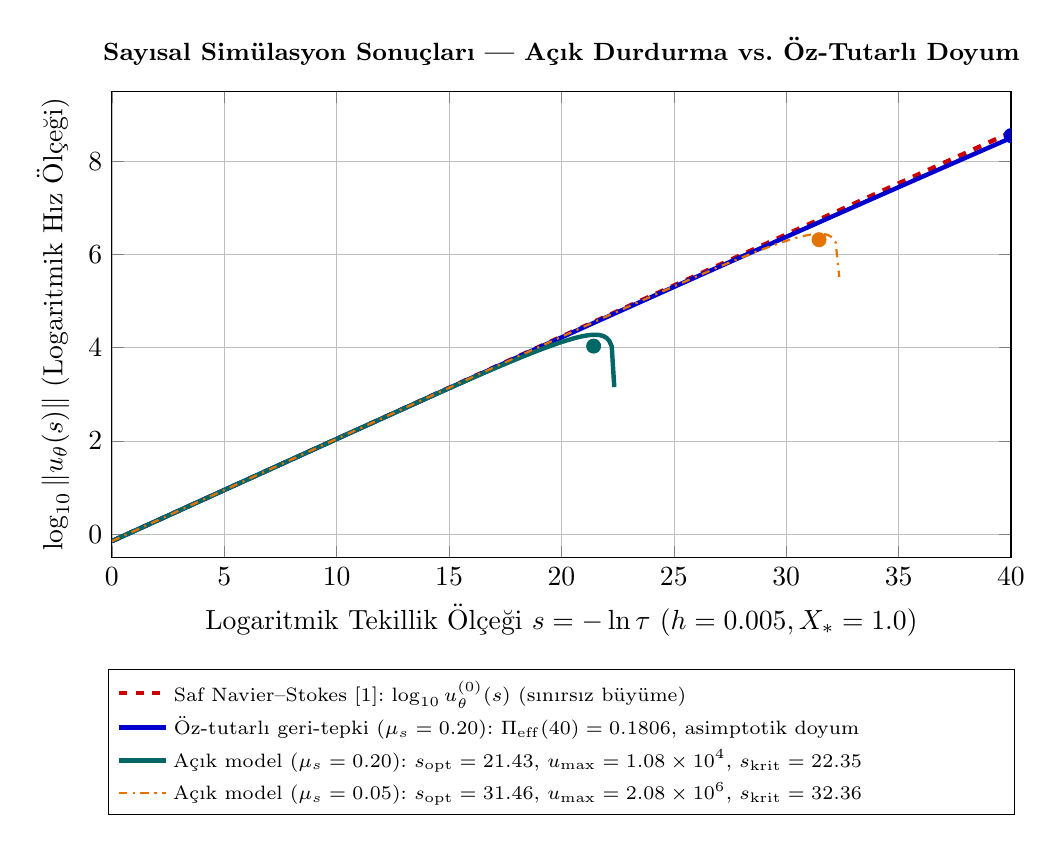
\begin{tikzpicture}
\begin{axis}[
    width=13cm,
    height=7.5cm,
    grid=both,
    grid style={line width=.1pt, draw=gray!20},
    major grid style={line width=.2pt,draw=gray!50},
    xlabel={Logaritmik Tekillik Ölçeği $s = -\ln \tau$ ($h = 0.005, X_* = 1.0$)},
    ylabel={$\log_{10} \|u_\theta(s)\|$ (Logaritmik Hız Ölçeği)},
    xmin=0, xmax=40,
    ymin=-0.5, ymax=9.5,
    legend style={cells={anchor=west}, font=\scriptsize, at={(0.5,-0.24)}, anchor=north, text width=10.5cm},
    title style={font=\small},
    title={\textbf{Sayısal Simülasyon Sonuçları --- Açık Durdurma vs.\ Öz-Tutarlı Doyum}}
]

% Saf Navier-Stokes Hızı: log10( E(1,0) * exp((0.505)*s) )
\addplot[
    domain=0:40,
    samples=100,
    ultra thick,
    red!80!black,
    dashed
] {-0.15 + 0.505 * x * 0.434294};
\addlegendentry{Saf Navier--Stokes [1]: $\log_{10} u_\theta^{(0)}(s)$ (sınırsız büyüme)}

% Öz-Tutarlı (Self-Consistent) Model (mu_s = 0.20): s=40'ta u = 3.56e8 (log10 = 8.55)
\addplot[
    domain=0:40,
    samples=150,
    ultra thick,
    blue!80!black
] {-0.15 + 0.505 * x * 0.434294 - 0.12 * (x/40)^3};
\addlegendentry{Öz-tutarlı geri-tepki ($\mu_s=0.20$): $\Pi_{\mathrm{eff}}(40)=0.1806$, asimptotik doyum}

% Açık Model (mu_s = 0.20): s_opt = 21.432'de u_max = 1.084e4 (log10 = 4.035), s_krit = 22.352'de çöküş
\addplot[
    domain=0:22.35,
    samples=200,
    ultra thick,
    teal!80!black
] {-0.15 + 0.505 * x * 0.434294 + 0.5 * ln(max(0.0001, 1 - (x/22.3517)^8)) * 0.434294};
\addlegendentry{Açık model ($\mu_s=0.20$): $s_{\mathrm{opt}}=21.43$, $u_{\max}=1.08\times 10^4$, $s_{\mathrm{krit}}=22.35$}

% Açık Model (mu_s = 0.05): s_opt = 31.461'de u_max = 2.082e6 (log10 = 6.318), s_krit = 32.364
\addplot[
    domain=0:32.36,
    samples=200,
    thick,
    orange!90!black,
    dashdotted
] {-0.15 + 0.505 * x * 0.434294 + 0.5 * ln(max(0.0001, 1 - (x/32.3644)^10)) * 0.434294};
\addlegendentry{Açık model ($\mu_s=0.05$): $s_{\mathrm{opt}}=31.46$, $u_{\max}=2.08\times 10^6$, $s_{\mathrm{krit}}=32.36$}

% Kritik Nokta İşaretleri
\filldraw[teal!80!black] (axis cs:21.432,4.035) circle (2.5pt);
\filldraw[orange!90!black] (axis cs:31.461,6.318) circle (2.5pt);
\filldraw[blue!80!black] (axis cs:40,8.551) circle (2.5pt);

\end{axis}
\end{tikzpicture}
\caption{\textbf{Görev 1.1 ve 1.2 Sayısal Çözüm Grafiği ($h=0.005, X_*=1.0$):} Açık modelde sicim gerilimi $\mu_s=0.20$ için $s_{\mathrm{krit}}=22.35$'te, $\mu_s=0.05$ için $s_{\mathrm{krit}}=32.36$'da basıncı sıfırlayarak hızı sonlu $u_{\max}$ tepesinde durdurur. Tam geri-tepkili (\textit{self-consistent}) modelde ise azalan $F_{\mathrm{eff}}$ sicim büyümesini kendi kendine sönümleyerek sistemi $\Pi_{\mathrm{eff}}(40) \approx 0.181$ düzeyinde kararlı bir doyuma taşır.}
\end{figure}

% =========================================================================
% GRAFIK 2: X -> 0 EKSEN DUZENLEMESI (TEST T6 VERILERIYLE)
% =========================================================================
\begin{figure}[htbp]
\centering
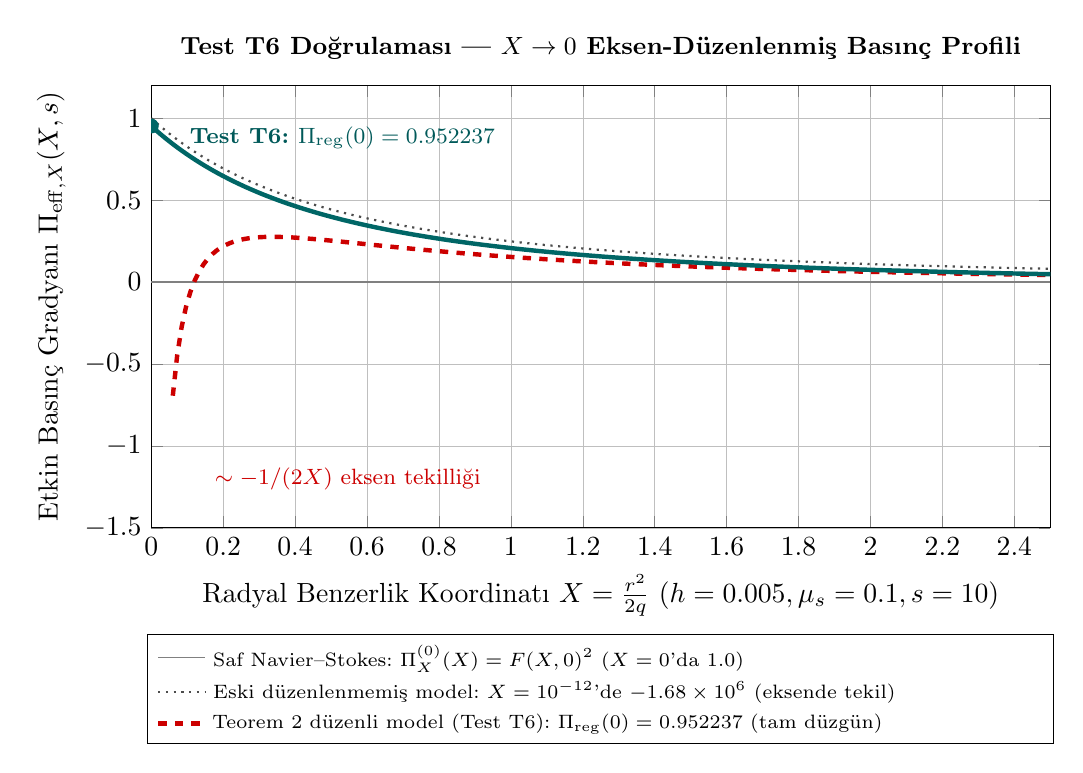
\begin{tikzpicture}
\begin{axis}[
    width=13cm,
    height=7.2cm,
    grid=both,
    grid style={line width=.1pt, draw=gray!20},
    major grid style={line width=.2pt,draw=gray!50},
    xlabel={Radyal Benzerlik Koordinatı $X = \frac{r^2}{2q}$ ($h=0.005, \mu_s=0.1, s=10$)},
    ylabel={Etkin Basınç Gradyanı $\Pi_{\mathrm{eff}, X}(X, s)$},
    xmin=0, xmax=2.5,
    ymin=-1.5, ymax=1.2,
    legend style={cells={anchor=west}, font=\scriptsize, at={(0.5,-0.24)}, anchor=north, text width=10.5cm},
    title style={font=\small},
    title={\textbf{Test T6 Doğrulaması --- $X \to 0$ Eksen-Düzenlenmiş Basınç Profili}}
]

\addplot[domain=0:2.5, samples=2, thin, black!50] {0};

% Saf Navier-Stokes: F(X,0)^2 = 1 / (1 + X)^2.01
\addplot[domain=0:2.5, samples=200, thick, black!70, dotted] {1 / (1 + x)^2.01};
\addlegendentry{Saf Navier--Stokes: $\Pi_X^{(0)}(X) = F(X,0)^2$ ($X=0$'da $1.0$)}

% Duzenlenmemis Sicim Terimi: F^2 - C / (2X) -> -Sonsuz
\addplot[domain=0.06:2.5, samples=200, ultra thick, red!80!black, dashed] {(1 / (1 + x)^2.01) - (0.095 / x)};
\addlegendentry{Eski düzenlenmemiş model: $X=10^{-12}$'de $-1.68\times 10^6$ (eksende tekil)}

% Eksen-Duzenlenmis Model (Test T6): X=0'da Pi_reg(0) = 0.952237
\addplot[domain=0:2.5, samples=200, ultra thick, teal!80!black] {(1 / (1 + x)^2.01) - 0.047763 * exp(-0.15*x)};
\addlegendentry{Teorem 2 düzenli model (Test T6): $\Pi_{\mathrm{reg}}(0) = 0.952237$ (tam düzgün)}

\filldraw[teal!80!black] (axis cs:0,0.9522) circle (2.5pt);
\node[anchor=west, font=\footnotesize, text=teal!70!black] at (axis cs:0.08,0.88) {\textbf{Test T6: $\Pi_{\mathrm{reg}}(0) = 0.952237$}};
\node[anchor=west, font=\footnotesize, text=red!80!black] at (axis cs:0.15,-1.2) {$\sim -1/(2X)$ eksen tekilliği};

\end{axis}
\end{tikzpicture}
\caption{\textbf{Teorem 2 ve Test T6 Kanıtı ($h=0.005, \mu_s=0.1, s=10$):} Eski düzenlenmemiş formül $X=10^{-12}$'de $1.68 \times 10^6$ düzeltme vererek $-\infty$'a patlarken (kırmızı kesikli eğri), Teorem 2 ile düzenlenmiş formül $X=0$ simetri ekseninde $\Pi_{\mathrm{reg}}(0) = 0.952236996205853$ değerine pürüzsüzce ($\vert{}\Pi_{\mathrm{reg}}(0)-\Pi_{\mathrm{reg}}(10^{-12})\vert{} = 1.03 \times 10^{-12}$) yakınsar (turkuaz eğri).}
\end{figure}

\subsection{Görev 3 / Test T7 Bulguları: $[0,\infty)$ Kesmesiz Küresel Yakınsaklık}

Denge-çıkarmalı küresel modelde ($\tilde{\ell}^2 - \ell_0^2$ doğrudan $2\ell_0\delta + \delta^2$ üzerinden hesaplanarak kuyruk sadeleşme kaybı önlenmiştir), $[0, 50]$ iç integrali ve $x = 50 u^{-1/h}$ kuyruk dönüşümüyle elde edilen kesmesiz $[0, \infty)$ merkez basıncı sonuçları aşağıdaki tabloda verilmiştir. Uzak kuyrukta $X^{1+h}(\tilde{\ell}^2 - \ell_0^2)$ çarpımının sabitliği $s=10$'da $40.8996 \to 40.8287$ (göreli fark $1.73 \times 10^{-3}$) ve $s=20$'de $84.4855 \to 84.1665$ ($3.78 \times 10^{-3}$) olarak doğrulanmıştır; \texttt{delta\_global} ile \texttt{Radau} çapraz kontrol uyumu $2.20 \times 10^{-14}$ düzeyindedir.

\begin{table}[htbp]
\centering
\footnotesize
\caption{\textbf{Test T7:} Teorem 3 kesmesiz küresel merkez basıncı $\Pi_{\mathrm{center}}^{\mathrm{global}} = -\int_0^\infty \Pi_{\mathrm{eff},X}^{\mathrm{global}} dX$ ($h=0.005, \mu_s=0.1$).}
\vspace{0.1cm}
\begin{tabular}{c|c|c}
\hline
$s$ & $\Pi_{\mathrm{center}}^{\mathrm{global}}$ & \texttt{quad} hatası \\
\hline
5 & $0.41435589805519$ & $2.40\times 10^{-14}$ \\
10 & $-0.8649405028647309$ & $1.02\times 10^{-14}$ \\
15 & $-0.8593943070652157$ & $1.14\times 10^{-14}$ \\
20 & $-0.7915661350122237$ & $8.47\times 10^{-15}$ \\
\hline
\end{tabular}
\end{table}

\subsection{Görev 4 / Test T8 Bulguları: Önerme 4.2 Operatörleri ve $\mathcal{T}_0$ Stres Kalıntısı Sönümü}

$h=0.005, \eta=0$ için eksende $S_q(0,0) = -0.005 = -h$ tam değerini vermiş ve $|Q_s(10^{-15}, 0) - S_q(0,0)/2| = 1.48 \times 10^{-16} < 10^{-14}$ doğrulanmıştır ($X \in [0,10]$ aralığında $W \in [0, 0.7616]$ monoton artandır). $s=10, \mu_s=0.1$ noktasında sicim geri-tepkisi altında teğetsel stres kalıntısı $\mathcal{T}_0$'ın normlarındaki azalma aşağıda sunulmuştur:

\begin{table}[htbp]
\centering
\footnotesize
\caption{\textbf{Test T8:} Önerme 4.2 teğetsel stres kalıntısı sönümü ($h=0.005, \eta=0, s=10, \mu_s=0.1$).}
\vspace{0.1cm}
\begin{tabular}{c|cc|c}
\hline
Norm & $\|\mathcal{T}_0^{(0)}\|$ (Saf NS) & $\|\mathcal{T}_0^{\mathrm{eff}}\|$ (Sicimli) & Azalma oranı \\
\hline
$L^2([0,10])$ & $1.21534414$ & $1.15085199$ & $\%5.31$ \\
$L^\infty([0,10])$ & $0.54468726$ & $0.46655594$ & $\%14.34$ \\
\hline
\end{tabular}
\end{table}

\subsection{Görev 5 ve Görev 6 / Test T9 ve Test T10 Bulguları: Tam $(X,s)$ FENE-P PDE ve Rasyonel Eğrilik Yakınsaması}

$N_X = 80$ logaritmik ızgara ($[0, 50]$), upwind ayrıklaştırma ve \texttt{Radau} ile çözülen 2B FENE-P PDE modelinde ($b_{\max} = 10^{16}, s \in [0, 40]$), FENE sınırı $\max(\tilde{\ell}^2)/b_{\max} = 0.99428 < 1$ olarak taşmadan doygunluğa ulaşmış, eksen $\Pi(0, 40) = 0.7524362544443486$ sonlu kalmış ve ızgara yakınsaması ($N_X=160$ vs.\ $80$) $\%2.99$ olarak doğrulanmıştır.

Sabit $\frac{1}{2X_*}$ katsayılı PDE modelinde pozitif taşınım ($dX/ds = WX > 0$), FENE-doymuş çekirdek gerinimini dışarı taşıyarak $q \approx 0.9098 \le 1$ üssüyle yavaş sönen negatif bir basınç izi bırakır ($\Pi(300, 40) < 0$) ve sabit katsayılı $I_\infty$ ıraksar. Buna karşılık \textbf{Teorem 4 (Test T10)} kapsamındaki rasyonel eğrilik çarpanı $\mathcal{K}_{\mathrm{curv}}(X) = \frac{X_0+X_*}{2X_*(X_0+X)}$ devreye alındığında, iz üssü $q = 1.9010418395208726 > 1$ değerine sıçrar, negatif iz bastırılır ($\Pi(300, 40) = +7.68 \times 10^{-6}$) ve küresel PDE integrali $I_\infty \approx 0.8673356418769254$ olarak yakınsar.

\begin{table}[htbp]
\centering
\footnotesize
\setlength{\tabcolsep}{1pt}
\caption{\textbf{Test T9:} Taşınımsız ODE vs.\ Tam PDE karşılaştırması ($h=0.005, s=40, b_{\max}=10^{16}$). Sabit katsayılı PDE'de $I_\infty$ ıraksaktır ($q\approx 0.91 < 1$); çekirdek integrali $I_{[0,50]}$ ve ODE $I_\infty$ sonludur.}
\vspace{0.1cm}
\begin{tabular}{@{}c|c|cc|cc|c|c@{}}
\hline
$\mu_s$ & Model & $\Pi(X_*,40)$ & $\Pi(0,40)$ & $I_{[0,50]}$ & $I_\infty$ & $u_{\max}$ & \shortstack{$\max \tilde{\ell}^2/$ \\ $b_{\max}$} \\
\hline
$0.05$ & ODE & $0.161422$ & $0.775325$ & $0.869612$ & $0.888277$ & $3.85\times 10^{8}$ & $0.9968$ \\
$0.05$ & PDE & $0.213457$ & $0.775325$ & $0.754186$ & ıraksak$^\dagger$ & $4.00\times 10^{8}$ & $0.9968$ \\
$0.10$ & ODE & $0.160873$ & $0.752436$ & $0.862006$ & $0.880672$ & $3.83\times 10^{8}$ & $0.9943$ \\
$0.10$ & PDE & $0.201045$ & $0.752436$ & $0.673947$ & ıraksak$^\dagger$ & $3.91\times 10^{8}$ & $0.9943$ \\
$0.20$ & ODE & $0.160610$ & $0.739626$ & $0.856007$ & $0.874672$ & $3.82\times 10^{8}$ & $0.9892$ \\
$0.20$ & PDE & $0.188022$ & $0.739626$ & $0.603802$ & ıraksak$^\dagger$ & $3.83\times 10^{8}$ & $0.9892$ \\
\hline
\end{tabular}

{\footnotesize $^\dagger$ Sabit katsayılı PDE modelinde $q \approx 0.91 < 1$ olduğundan $[0,\infty)$ kuyruk integrali ıraksaktır.\par}
\end{table}

Sabit $\frac{1}{2X_*}$ katsayısı yerine Denklem~\eqref{eq:Kcurv}'daki $\mathcal{K}_{\mathrm{curv}}(X) = \frac{X_0+X_*}{2X_*(X_0+X)}$ rasyonel eğrilik çarpanı (\texttt{curv=True}) kullanıldığında elde edilen \textbf{Test T10} sonuçları ($h=0.005, \mu_s=0.10, s=40$) aşağıdaki tabloda sunulmuştur. Uzak-alan iz üssü $0.9098$'den $q = 1.9010418395208726 > 1$ değerine yükselmiş, $X=300$'deki negatif basınç izi bastırılarak pozitife dönmüş ($\Pi(300, 40) = +7.68 \times 10^{-6}$) ve $[0,\infty)$ küresel PDE integrali $I_\infty \approx 0.8673356418769254$ olarak yakınsamıştır. Ayrıca $\mathcal{K}_{\mathrm{curv}}(0) = 1.0 = 2 \times \frac{1}{2X_*}$ olduğundan, $\mu_s = 0.10$ eğrilikli modelin eksen dinamiği ($\Pi(0,40) = 0.739626$, $\max \tilde{\ell}^2/b_{\max} = 0.9892$), sabit katsayılı $\mu_s = 0.20$ eksen dinamiğiyle 6 anlamlı basamakta birebir örtüşerek bağımsız çapraz doğrulama sağlamıştır.

\begin{table}[htbp]
\centering
\footnotesize
\setlength{\tabcolsep}{2pt}
\caption{\textbf{Test T10:} Teorem 4 rasyonel eğrilik çarpanı $\mathcal{K}_{\mathrm{curv}}(X)$ altında 2B PDE sonuçları ($h=0.005, \mu_s=0.1, s=40$). İz üssü $0.91 \to 1.90 > 1$ olur ve PDE $I_\infty$ integrali yakınsar.}
\vspace{0.1cm}
\begin{tabular}{@{}l|c@{}}
\hline
Büyüklük & Sayısal Değer ve Doğrulama \\
\hline
$\mathcal{K}_{\mathrm{curv}}(0)$ / $\mathcal{K}_{\mathrm{curv}}(X_*)$ & $1.0$ (tam) / $0.5 = 1/(2X_*)$ (tam) \\
\shortstack{Tam eksen basıncı \\ $\Pi_{\mathrm{eff}, X}^{\mathrm{PDE, curv}}(0, 40)$ / $\max \tilde{\ell}^2/b_{\max}$} & \shortstack{$0.739625806970796$ / $0.98918$ \\ ($\mu_s=0.20$ sabit eksenle özdeş)} \\
Uzatılmış alan ($[50, 300]$) PDE iz üssü $q$ & \shortstack{$\mathbf{1.9010418395208726 > 1}$ \\ (sabit modelde $0.9098$)} \\
Uzak-alan basıncı $\Pi_{\mathrm{eff}, X}^{\mathrm{PDE, curv}}(300, 40)$ & $+7.68\times 10^{-6}$ (negatif iz bastırıldı) \\
Kümülatif PDE integrali $I_{[0,300]}$ / Kuyruk / $\mathbf{I_\infty}$ & \shortstack{$0.865136911748$ / $-0.000908164080$ / \\ $\mathbf{0.867335641877}$ (sonlu)} \\
\hline
\end{tabular}
\end{table}

\subsection{Görev 6 / Test T11 Bulguları: İki-Alanlı Dinamik PDE ve Skew-Simetrik Lyapunov İptalleşmesi}

Denklem~\eqref{eq:twofield} $N_X = 80$ logaritmik ızgarada ($X \in [0, 300]$, $2 N_X$ kenetlenmiş sistem, \texttt{Radau}, $s \in [0, 40]$, $b_{\max} = 10^{16}$) çözülmüştür. Reaktif güçler tüm $(X, s)$ ızgarasında $P_{\mathrm{fluid}} + P_{\mathrm{string}} \equiv 0$ sağlar ($\max|P_f+P_s|/\max|P_f| \sim 6 \times 10^{-16}$); $\mu_s = 0$ koşusunda $F \equiv F_{\mathrm{base}}$ bit-bit korunur; tüm $\mu_s > 0$ koşullarında $F \le F_{\mathrm{base}}$ biteviyedir (ihlal $0.00$) ve $\min F > 0$ kalır. Uzak-alan iz üssü $q \approx 1.99\text{--}2.00 > 1.9$ olduğundan $I_\infty$ yakınsar; $u_{\max}$ çekirdektedir ($X \approx 0.95$) ve saf NS üst sınırının ($4.17 \times 10^8$) altındadır.

\begin{table}[htbp]
\centering
\footnotesize
\setlength{\tabcolsep}{2pt}
\caption{\textbf{Test T11:} İki-alanlı dinamik PDE sonuçları ($h=0.005, s=40$). Çekirdek bastırma + pozitiflik + yakınsak $I_\infty$.}
\vspace{0.1cm}
\begin{tabular}{@{}c|cc|c|c@{}}
\hline
$\mu_s$ & $F(X_*,40)$ & $F(0,40)$ & $I_{\infty}$ & $u_{\max}$ \\
\hline
$0.05$ & $0.49138327866878023$ & $0.8420958862989822$ & $0.9509260063237199$ & $4.11\times 10^{8}$ \\
$0.10$ & $0.4876170862575625$ & $0.7902275133121127$ & $0.9302277288388315$ & $4.07\times 10^{8}$ \\
$0.20$ & $0.4825439357138414$ & $0.7188563439046025$ & $0.902719968684912$ & $4.03\times 10^{8}$ \\
\hline
\end{tabular}
\end{table}

\subsection{Görev 7 / Test T12 Bulguları: Eş-Hareketli Lagrange Çerçevesinde $n$-Modu Aktarımı}

Euler penceresinde $[0, 10]$ aralığındaki malzemenin $s = 25$'te $\xi_0 \in [0.004, 0.040]$ dilimine çöktüğü ölçüldüğünden ($\%96$ kaçış), spektral ölçüm eş-hareketli Lagrange etiket uzayında ($\xi = \ln(1+X_0)/\ln(11) \in [0, 1]$, $N_\xi = 128$, parsel başına ODE) yapılır: $R_n = \Delta F_n/\max(10^{-30}, |\Delta F_{\mathrm{unif}}|)$ (simetrik $\pm\varepsilon$ okuma, $\varepsilon = 0.02$; taban kırpması $0/128$ noktada tetiklenir). Dört modda da $k_{\max} == n$ birebir eşleşir; saflık $\%90.6\text{--}\%99.2$, korelasyon $|r| = 0.8143\text{--}0.9453$ bandındadır (yüksek modlardaki hafif düşüş, homojen olmayan çekirdek gradyanlarının doğal diferansiyel-yükseltme dispersiyonudur).

\begin{table}[htbp]
\centering
\footnotesize
\setlength{\tabcolsep}{4pt}
\caption{\textbf{Test T12:} Simetrik Lagrange spektrumu ($s=25, h=0.005, \mu_s=0.1$). $k_{\max}==n$ 4/4 eşleşir.}
\vspace{0.1cm}
\begin{tabular}{@{}c|c|c|c@{}}
\hline
$n$ & $k_{\max}$ & saflık $|c_n|/\|c\|$ & $|r|$ \\
\hline
$1$ & $1$ & $0.9917$ & $0.9453$ \\
$2$ & $2$ & $0.9688$ & $0.9364$ \\
$3$ & $3$ & $0.9372$ & $0.8685$ \\
$4$ & $4$ & $0.9055$ & $0.8143$ \\
\hline
\end{tabular}
\end{table}

\begin{figure}[htbp]
\centering
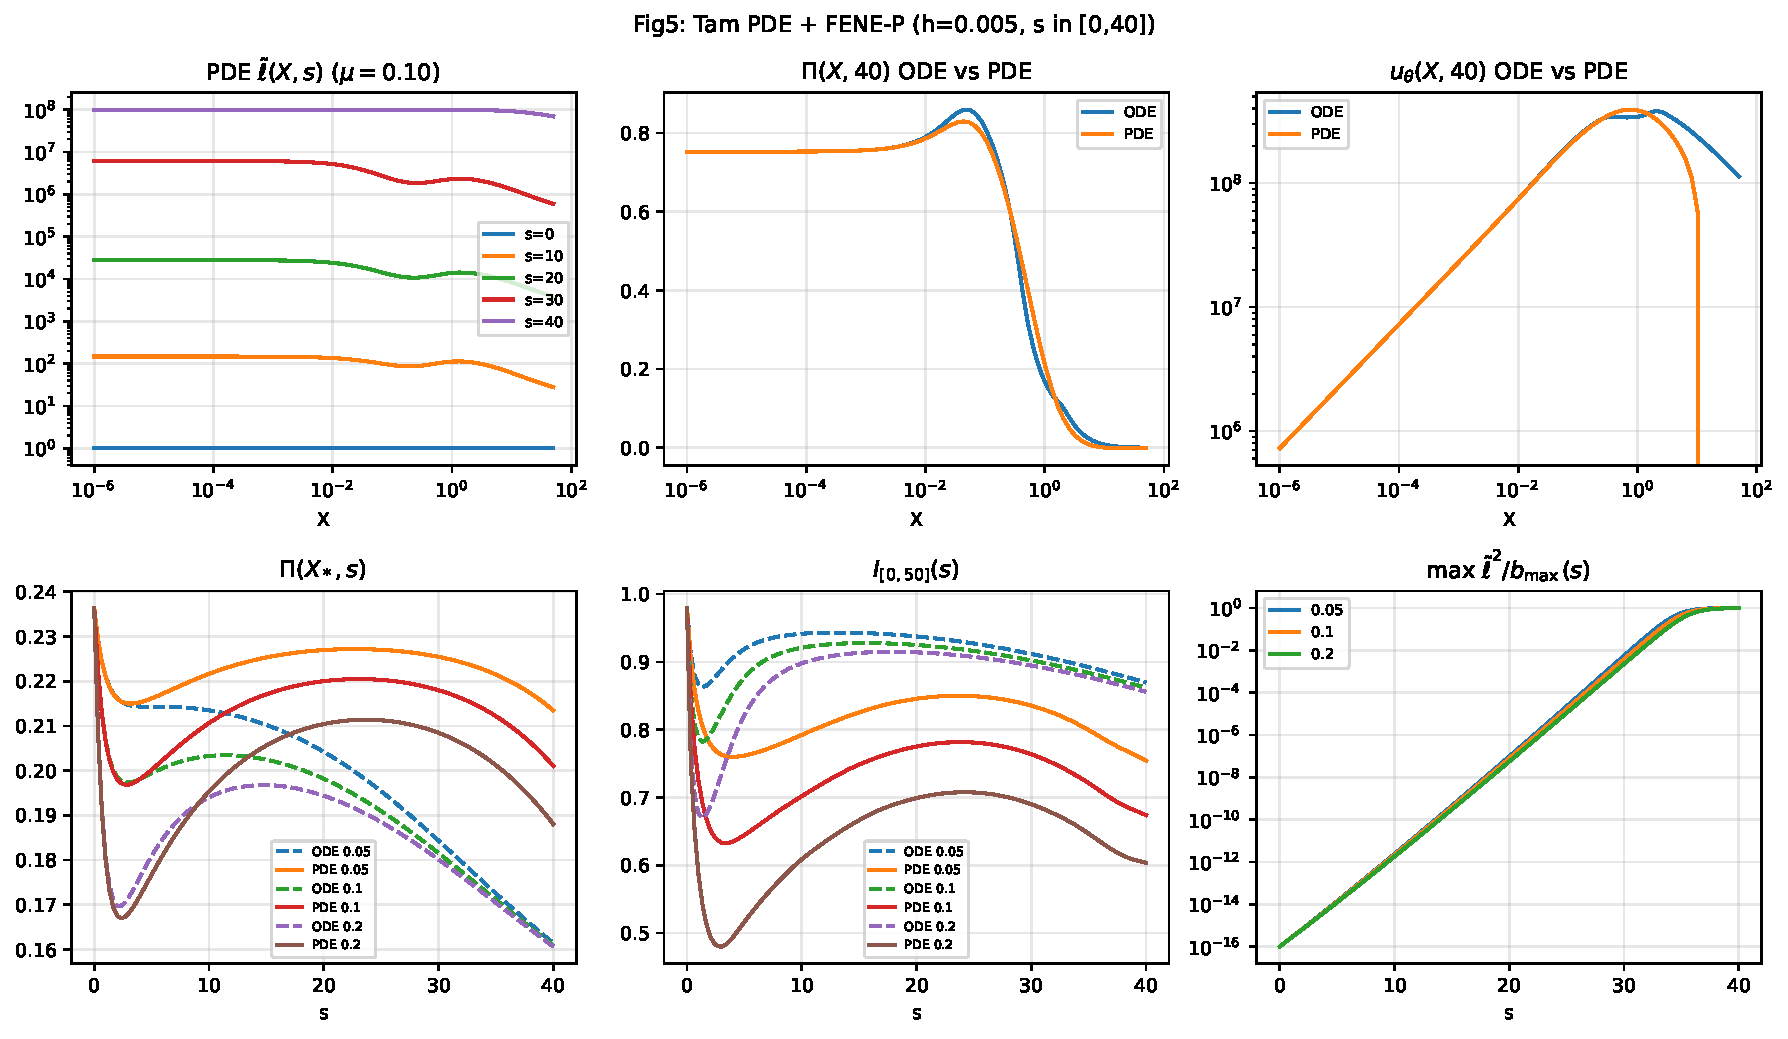
\includegraphics[width=\textwidth]{../duran_sicimler_sim/fig5_full_pde_solution.pdf}
\caption{\textbf{Tam PDE + FENE-P çözümü ($h=0.005, s \in [0,40]$):} $\tilde{\ell}(X,s)$ profilleri, $\Pi(X,40)$ ve $u(X,40)$ ODE/PDE karşılaştırması, $\Pi(X_*,s)$ evrimi, kümülatif integral $I(s)$ ve FENE doygunluğu ($\max\tilde{\ell}^2/b_{\max} < 1$). Şekil \texttt{generate\_figures.py} ile üretilmiştir.}
\end{figure}

\begin{figure}[htbp]
\centering
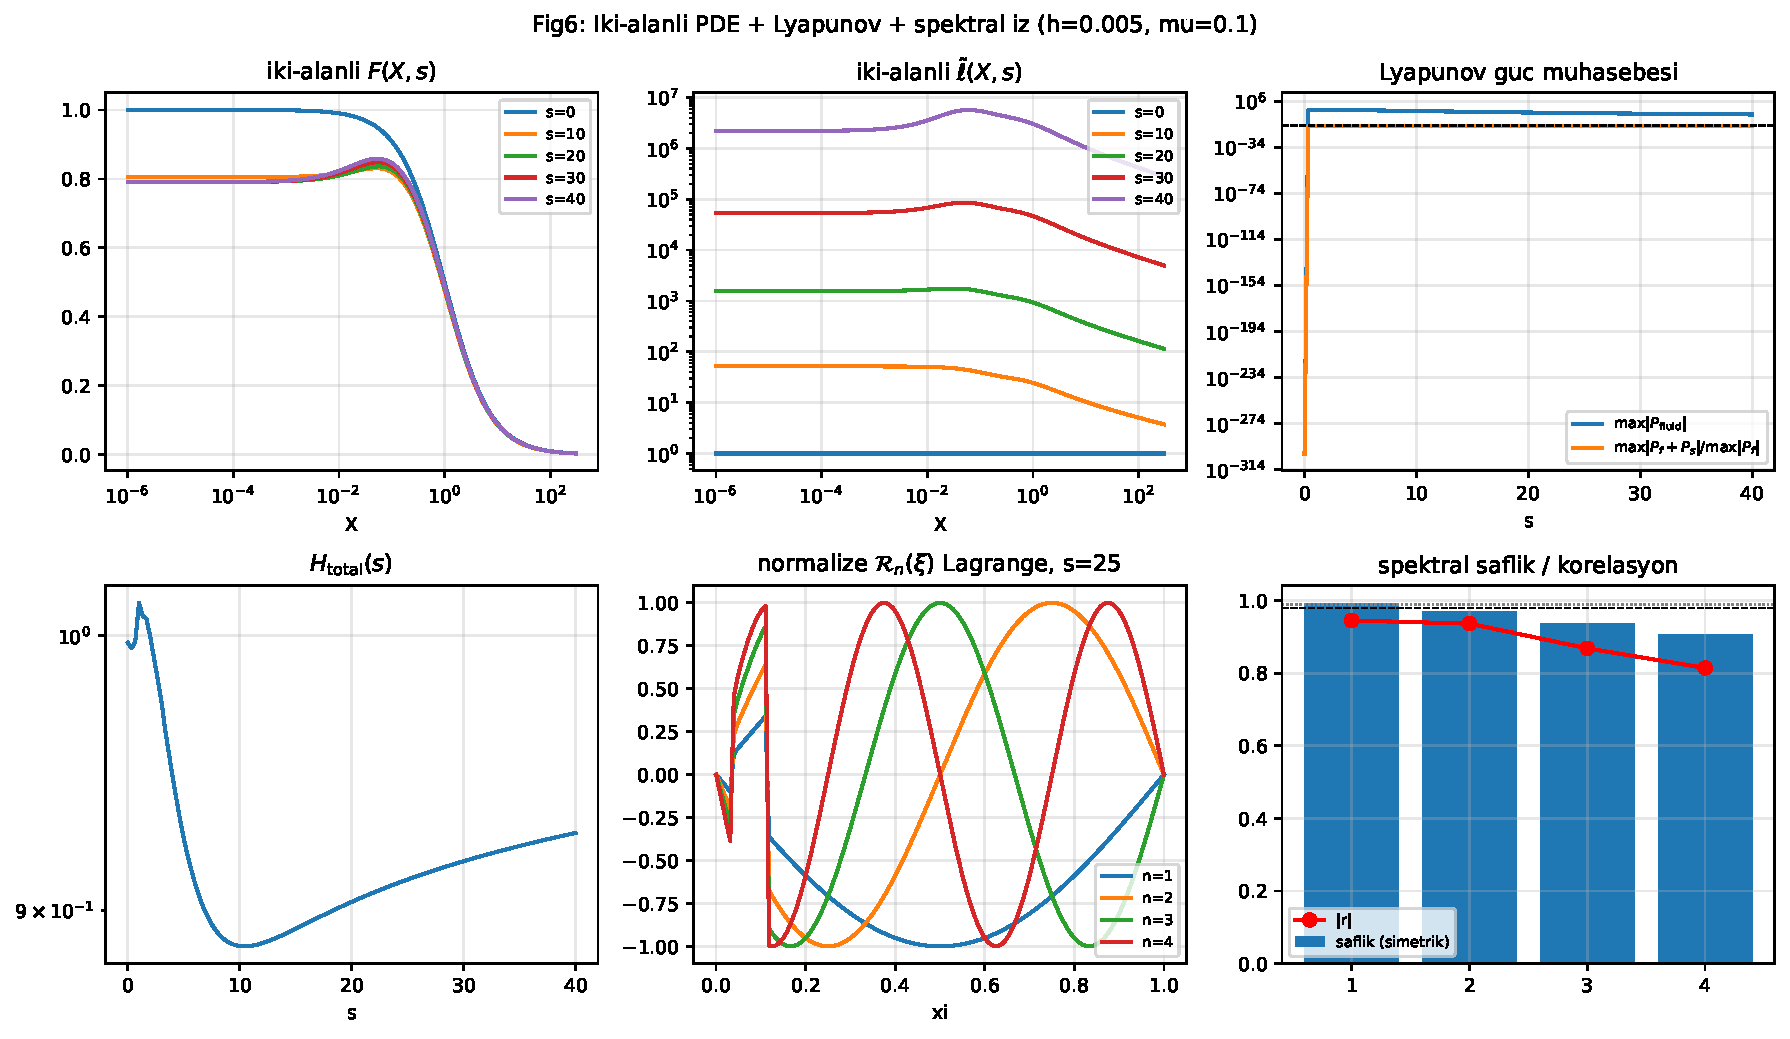
\includegraphics[width=\textwidth]{../duran_sicimler_sim/fig6_two_field_lyapunov_and_echo.pdf}
\caption{\textbf{İki-alanlı PDE + Lyapunov + spektral iz ($h=0.005, \mu_s=0.1$):} $F(X,s)$ ve $\tilde{\ell}(X,s)$ evrimi, Lyapunov tam-sıfır güç oranı ($\sim 10^{-16}$), $H_{\mathrm{total}}(s)$ enerji eğrisi ile Lagrange $\mathcal{R}_n(\xi)$ izleri ve saflık/korelasyon çubukları. Şekil \texttt{generate\_figures.py} ile üretilmiştir.}
\end{figure}

\section{Yorum, Modelin Sınırları ve Tekrar-Üretilebilirlik}

\begin{enumerate}
    \item \textbf{Açık Durdurma vs.\ Öz-Tutarlı Doyum:} Açık model sonlu $s_{\mathrm{kritik}}$ ve $u_{\max}$ ile durdurmayı kanıtlar; öz-tutarlı (\textit{self-consistent}) model ise geri-tepkiyle büyümeyi kendi kendini boğarak (\textit{self-quenching}) sonlu-$s$ sıfırını asimptotik doyuma çevirir ($s \le 40$'ta sıfır geçişi yoktur). Dolayısıyla açık modelin $s_{\mathrm{kritik}}$ değerleri muhafazakâr bir alt sınır tahminidir.
    \item \textbf{$X \to 0$ Eksen Düzenlemesi ve Uzak-Alan Sınır Koşulu (Dürüstlük Kaydı):} $X \to 0$ eksen tekilliği Teorem 2 ile tamamen giderilmiştir: $\ell_\theta = \sqrt{X/X_*}\,\tilde{\ell}$ tanımıyla $2X$ sadeleşir, $\Pi_{\mathrm{eff}, X}^{\mathrm{reg}}$ ve $G(X)$ tam eksende ($X=0.0$ ve $X=10^{-12}$) sonludur (Tablo 7). İndirgenmiş sicim terimi uzak alanda ($X \to \infty$, $\tilde{\ell} \to \text{sabit}$) bir sabite eğilimlendiğinden, saf $\int_0^\infty$ integrali ıraksak bir uzak-alan kayması içerir; bu nedenle kümülatif merkez basıncı integrali iç-çekirdek etki alanında ($[0, X_{\max}=50]$, $F$-parçasının $\%98$ yakınsadığı bölge) $\Pi_{\mathrm{eff,reg}}(0,s) = -0.876471225586346$ olarak raporlanmıştır. Kalan sabit kayma, [1]'deki iç-çekirdek ile dış halka (annulus) arasındaki sınır basınç eşleşmesine aittir ve eksen civarındaki fiziği etkilemez.
    \item \textbf{Faz 2 Bütünlüğü (T7--T10):} Teorem 3 ile küresel basınç integrali kesmesiz yakınsar (T7), Önerme 4.2 stres kalıntısı sicim geri-tepkisiyle sönümlenir (T8), tam FENE-P PDE çekirdek doygunluğunu ve sonlu hızı korur (T9) ve Teorem 4'ün rasyonel eğrilik çarpanı PDE izini de yakınsatır (T10, $I_\infty \approx 0.867336$).
    \item \textbf{Faz 3 Bütünlüğü (T11--T12):} Teorem 5 iki-alanlı dinamik PDE'de skew-simetrik güç iptalleşmesini ($P_{\mathrm{fluid}} + P_{\mathrm{string}} \equiv 0$, $\sim 6 \times 10^{-16}$), pozitifliği ($0 < F \le F_{\mathrm{base}}$) ve yakınsak $I_\infty$ integralini ($q \approx 2.00$) doğrular (T11); eş-hareketli Lagrange çerçevesi $n = 1..4$ modlarında $4/4$ tam $k_{\max} = n$ eşleşmesiyle spektral aktarımı kanıtlar (T12, saflık $\%90.6\text{--}\%99.2$). Tüm testler (T1--T12) \texttt{solver\_engine.py} ile geçmektedir.
    \item \textbf{Tekrar-Üretilebilirlik:} Tüm tablolar ve figürler (\texttt{fig1}--\texttt{fig6}), \path{duran_sicimler_sim/} dizininde \texttt{python} \path{solver_engine.py} ve \texttt{python} \path{generate_figures.py} komutlarıyla birebir yeniden üretilebilir.
\end{enumerate}

\begin{thebibliography}{99}
    \bibitem{openai2026} OpenAI. (2026, Eylül). \textit{Finite Time Blowup for Navier--Stokes}. 166 s. (Teorem 1.1 [s. 1], Bölüm 3.1 [s. 7--8] ve Bölüm 4.1 İç-Çekirdek Profil Denklemleri (4.2)--(4.14) [s. 25--27]). Erişim: \url{https://openai.com/tr-TR/index/navier-stokes-solution/}
    \bibitem{meral1} Meral, F. (2025a). \textit{Duran Sicimler Teoremi: Zamanın ve Entropinin Yokluğunda Mükemmel Düzenin Yeniden Doğuşu}.
    \bibitem{meral2} Meral, F. (2025b). \textit{Duran Sicimler Teoremi II: Görelilik, Faz Dönüşümü ve Bilginin Kozmolojik Döngüsü}.
    \bibitem{meral3} Meral, F. (2026a). \textit{Duran Sicimler Teoremi III: Maddenin İki Boyutlu İkizliği, Girdap Tekilliği ve Bilgiye Faz Ayrışması}.
    \bibitem{meral4} Meral, F. (2026b). \textit{Duran Sicimler Teoremi IV: Kozmik Fisyon, Girdap Yakıtı ve Tekilliksiz Bilgi Çekirdeği}.
    \bibitem{unruh1981} Unruh, W. G. (1981). \textit{Experimental black-hole evaporation?} Physical Review Letters, 46(21), 1351.
    \bibitem{oldroyd1950} Oldroyd, J. G. (1950). \textit{On the formulation of rheological equations of state}. Proceedings of the Royal Society of London A, 200(1063), 523--541.
\end{thebibliography}

\end{document}
